%% ============================================================
%%  Bachelor-Thesis – Hochschule Heilbronn
%%  
%%  
%% ============================================================

\documentclass[
  12pt,
  a4paper,
  oneside,
  openright,
  listof=totoc,
  bibliography=totoc,
  parskip=half          % Absätze durch Leerzeile statt Einrückung
]{scrreprt}

%% ---- Präambel laden ----------------------------------------
%% ============================================================
%%  preamble.tex – Pakete & Konfiguration
%%  Hochschule Heilbronn | Bachelor-Thesis
%% ============================================================

%% ---- Sprache & Encoding ------------------------------------
\usepackage[utf8]{inputenc}
\usepackage[T1]{fontenc}
\usepackage[ngerman]{babel}
\usepackage{csquotes}      
\usepackage{physics}

% \enquote{} für korrekte Anführungszeichen

%% ---- Schrift -----------------------------------------------
\usepackage{lmodern}
\usepackage{microtype}            % Besserer Textsatz, weniger Overfull hboxes

%% ---- Seitenlayout ------------------------------------------
%  HHN-Norm: links 3cm (Bindung), rechts 2.5cm, oben/unten 2.5cm
\usepackage[
  a4paper,
  left=3cm,
  right=2.5cm,
  top=2.5cm,
  bottom=2.5cm,
  bindingoffset=5mm
]{geometry}

%% ---- Zeilenabstand -----------------------------------------
\usepackage{setspace}
\onehalfspacing

%% ---- Kopf- & Fußzeilen (KOMA) ------------------------------
\usepackage[
  headsepline,
  automark
]{scrlayer-scrpage}
\pagestyle{scrheadings}
\automark[section]{chapter}
\clearpairofpagestyles
\ihead{\headmark}
\ohead{\pagemark}
\cfoot{}
% Kapitelseiten erhalten dieselbe Kopfzeile
\renewcommand*{\chapterpagestyle}{scrheadings}

%% ---- Grafik & Abbildungen ----------------------------------
\usepackage{graphicx}
\graphicspath{{figures/}}
\usepackage{float}
\usepackage{caption}
\captionsetup{
  font=small,
  labelfont=bf,
  format=hang
}
\usepackage{subcaption}
\usepackage{multirow}


%% ---- Tabellen ----------------------------------------------
\usepackage{booktabs}             % \toprule, \midrule, \bottomrule
\usepackage{tabularx}
\usepackage{longtable}
\usepackage{array}

%% ---- Mathematik --------------------------------------------
\usepackage{amsmath}
\usepackage{amssymb}
\usepackage{eurosym}
%% ---- Quellcode (Listings) ----------------------------------
\usepackage{listings}
\usepackage{xcolor}
\usepackage{graphicx}
\usepackage{minted} 

\definecolor{lstbg}{gray}{0.97}
\definecolor{lstcomment}{rgb}{0.13,0.55,0.13}
\definecolor{lstkeyword}{rgb}{0.0,0.0,0.75}
\definecolor{lststring}{rgb}{0.63,0.13,0.13}

\lstset{
  backgroundcolor=\color{lstbg},
  basicstyle=\ttfamily\small,
  keywordstyle=\color{lstkeyword}\bfseries,
  commentstyle=\color{lstcomment}\itshape,
  stringstyle=\color{lststring},
  numbers=left,
  numberstyle=\tiny\color{gray},
  numbersep=8pt,
  frame=single,
  framerule=0.4pt,
  rulecolor=\color{gray!40},
  breaklines=true,
  breakatwhitespace=true,
  captionpos=b,
  tabsize=2,
  showstringspaces=false
}

%% ---- Abkürzungsverzeichnis ---------------------------------
\usepackage{acronym}

%% ---- Literaturverwaltung (BibLaTeX + Biber) ----------------
\usepackage[
  backend=biber,
  style=ieee,       % Autor-Jahr-Stil (Harvard)
  % style=numeric         % Nummern-Stil [1], [2], ...
  % style=ieee            % IEEE-Stil
  sorting=nyt,
  maxbibnames=99,
  maxcitenames=2,
  giveninits=true,
  uniquename=init
]{biblatex}
\addbibresource{literatur.bib}

%% ---- Hyperlinks & PDF-Metadaten ----------------------------
\usepackage[
  colorlinks=true,
  linkcolor=black,
  citecolor=black,
  urlcolor=blue,
  bookmarksnumbered=true,
  pdfborder={0 0 0}
]{hyperref}
\usepackage{bookmark}

%% ---- Hilfspackages -----------------------------------------
\usepackage{lipsum}               % Blindtext zum Testen → später entfernen


%% --- Code-----------------------------------------------------


\lstdefinestyle{python}{
  language=Python,
  basicstyle=\ttfamily\small,
  keywordstyle=\color{blue!70!black},
  stringstyle=\color{green!40!black},
  commentstyle=\color{gray}\itshape,
  numbers=left,
  numberstyle=\tiny\color{gray},
  numbersep=8pt,
  frame=single,
  rulecolor=\color{gray!40},
  backgroundcolor=\color{gray!5},
  breaklines=true,
  showstringspaces=false,
  captionpos=b,
  extendedchars=true,
  literate={ä}{{\"a}}1 {ö}{{\"o}}1 {ü}{{\"u}}1 {Ä}{{\"A}}1 {Ö}{{\"O}}1 {Ü}{{\"U}}1 {ß}{{\ss}}1
}
\lstset{style=python}

%% ---- Metadaten  -----------------------------
\newcommand{\ThesisTitel}{Entwicklung und Benchmarking einer Abstraktionsschicht für Quanten-Software}
\newcommand{\ThesisAutor}{Daniel Faigle}
\newcommand{\ThesisMatrikel}{215467}
\newcommand{\ThesisStudiengang}{Software Engineering}
\newcommand{\ThesisFakultaet}{Informatik}
\newcommand{\ThesisErstpruefer}{Prof. Dr. rer. nat. David Kreplin
(Hochschule Heilbronn)}
\newcommand{\ThesisZweitpruefer}{M.Sc. Moritz Willmann (Fraunhofer IPA)}
\newcommand{\ThesisUnternehmen}{Fraunhofer-Institut IPA}  
\newcommand{\ThesisZeitraum}{1.04.2026 - 03.08.2026}
\newcommand{\ThesisDatum}{August 2026}


%% ============================================================
\begin{document}

%% ---- Titelseite --------------------------------------------

\begin{titlepage}
  \newgeometry{left=3cm, right=2.5cm, top=2cm, bottom=2cm}

  %% -- HHN Logo oben rechts --
  \begin{minipage}[c]{0.48\textwidth}
    
\includegraphics[width=4.5cm]{figures/fraunhofer_ipa.jpg}
  \end{minipage}%
  \begin{minipage}[c]{0.48\textwidth}
    \raggedleft
    
\includegraphics[width=4.5cm]{figures/hhn}
  \end{minipage}

  \vspace{3cm}



  %% -- Typ der Arbeit --
  \begin{center}
    {\Large \textbf{Bachelor Thesis}}\\[0.4cm]
        {\large Hochschule Heilbronn  Fakultät für \ThesisFakultaet}\\[0.3cm]
    {\normalsize Bachelor of Science (B.\,Sc.) \ThesisStudiengang}
  \end{center}

  \vspace{1.5cm}

  %% -- Titel --
  \begin{center}
    {\LARGE \textbf{\ThesisTitel}}\\[0.5cm]
  \end{center}

  \vspace{2cm}

  %% -- Angaben zum Autor --
  \begin{center}
    {\normalsize vorgelegt von}\\[0.5cm]
    {\large \textbf{\ThesisAutor}}\\[0.2cm]
    {\normalsize Matrikelnummer: \ThesisMatrikel}
  \end{center}

  \vfill

  %% -- Prüfer & Datum --
  \begin{center}
    \begin{tabular}{ll}
      \textbf{Partnerunternehmen:}    & \ThesisUnternehmen\\[0.3cm]
      \textbf{Erstprüfer:}     & \ThesisErstpruefer \\[0.3cm]
      \textbf{Zweitprüfer:}    & \ThesisZweitpruefer \\[0.3cm]
      \textbf{Zeitraum:}    & \ThesisZeitraum \\[0.3cm]

      
    \end{tabular}
  \end{center}

  \restoregeometry
\end{titlepage}
\cleardoublepage


%% ---- Front Matter (römische Seitenzahlen) ------------------
\pagenumbering{Roman}

%\chapter*{Sperrvermerk}
\addcontentsline{toc}{chapter}{Sperrvermerk}

Die vorliegende Bachelor-Thesis mit dem Titel \enquote{\ThesisTitel}
enthält vertrauliche Informationen und Daten der Firma \ThesisUnternehmen.
Die Arbeit ist daher für die öffentliche Nutzung gesperrt.

Veröffentlichung, Vervielfältigung und Einsichtnahme – auch in Auszügen – sind
ohne ausdrückliche schriftliche Genehmigung des Unternehmens nicht gestattet.
Die Thesis darf nur den Gutachtern und den zuständigen Mitgliedern des
Prüfungsausschusses zugänglich gemacht werden.

\vspace{2cm}
\noindent
Heilbronn, \ThesisDatum
\hfill
\begin{minipage}{6cm}
  \centering
  \rule{5.5cm}{0.4pt}\\[0.2cm]
  \ThesisAutor
\end{minipage}

\cleardoublepage

%\chapter*{Danksagung}
\addcontentsline{toc}{chapter}{Danksagung}


\cleardoublepage


%% ============================================================
%%  00_abstract.tex – Abstract & Zusammenfassung
%% ============================================================
\chapter*{Abstract}
\addcontentsline{toc}{chapter}{Abstract}
% English summary (approx. 150–250 words).
This bachelor's thesis addresses the development and runtime analysis of an
abstraction layer that allows quantum circuits and observables to be described in a
single form and subsequently executed as objects of the quantum frameworks
\textit{PennyLane} and \textit{Qiskit}. The software component was integrated into
the \textit{Executor} Python library, which is currently under active development at
Fraunhofer IPA and is to be published under an open-source license in the near
future. Its previous internal representation relied on \textit{Qiskit} objects and
was therefore tied to a single framework. This dependency is replaced by a
self-contained data structure, so that the description of the circuit remains
unchanged and the execution environments of the respective other framework can be
addressed solely by selecting the backend. Since framework calls occur exclusively
within the backends, a program written once also remains executable across framework
version changes. In addition, the runtime overhead introduced by this layer compared
to direct use of the frameworks is evaluated.
\cleardoublepage

%% ---- Deutsche Zusammenfassung -----------------------------
\chapter*{Zusammenfassung}
\addcontentsline{toc}{chapter}{Zusammenfassung}
% Kurze Zusammenfassung auf Deutsch (ca. 150–250 Wörter).
Diese Bachelorarbeit befasst sich mit der Entwicklung und der Laufzeitanalyse einer
Abstraktionsschicht, über die sich Quantenschaltkreise und Observablen einheitlich
beschreiben und anschließend in den Objekten der Quantenframeworks
\textit{PennyLane} und \textit{Qiskit} ausführen lassen. Die Softwarekomponente
wurde in die Python-Softwarebibliothek \textit{Executor} integriert, die derzeit vom
Fraunhofer IPA aktiv weiterentwickelt wird und in naher Zukunft unter einer
Open-Source-Lizenz veröffentlicht werden soll. Bislang stützte sich deren interne
Darstellung auf \textit{Qiskit}-Objekte und war damit an ein einzelnes Framework
gebunden. Diese Bindung wird durch eine eigenständige Datenstruktur ersetzt, sodass
die Beschreibung des Schaltkreises unverändert bleibt und sich allein durch die
Auswahl des Backends die Ausführungsumgebungen des jeweils anderen Frameworks
ansprechen lassen. Da Framework-Aufrufe ausschließlich innerhalb der Backends
auftreten, bleibt ein einmal geschriebenes Programm zudem über Versionswechsel der
Frameworks hinweg lauffähig. Ergänzend wird der zeitliche Mehraufwand bewertet, den
diese Schicht gegenüber der direkten Nutzung der Frameworks verursacht.
\cleardoublepage

\tableofcontents
%\listoffigures
%\listoftables

%%\include{chapters/00_abkuerzungen}

%% ---- Hauptteil (arabische Seitenzahlen) --------------------
\pagenumbering{arabic}

\chapter{Einleitung}
\label{chap:einleitung}
Mit dem Gedankenexperiment einer Katze, die zugleich lebendig und tot ist, veranschaulichte Erwin Schrödinger 1935~\cite{schroedinger1935} eine der verblüffendsten Konsequenzen der Quantenmechanik. Phänomene der Quantenphysik wie die Superposition, bei der sich ein Teilchen gleichzeitig in mehreren Zuständen befinden kann, oder die Verschränkung, durch die Teilchen über beliebige Distanzen hinweg miteinander korreliert bleiben, widersprechen der Alltagserfahrung grundlegend. Genau von diesen Effekten erhofft man sich im Bereich des Computings einen fundamentalen Fortschritt~\cite{Taherdoost2025}. Das entsprechende Feld nennt sich Quantencomputing und nutzt die Superposition, um Systeme zu bauen, deren kleinste Recheneinheiten nicht nur die klassischen Zustände 0 und 1 annehmen können, sondern beide zugleich.

Die Forschung an Quantencomputern hat in den vergangenen Jahren erheblich an Aufschwung gewonnen. Sowohl große Technologiekonzerne wie IBM, Google und Microsoft als auch spezialisierte Unternehmen wie IonQ oder D-Wave und zahlreiche Universitäten investieren beträchtliche Mittel in die Entwicklung leistungsfähiger Quantensysteme und Quantensoftware~\cite{gibney2019quantum,bova2021commercial}. Auch staatliche Stellen stufen die Entwicklung von Quantencomputern als strategisch relevant ein. Der Bund stellte seit 2017 rund eine Milliarde Euro allein für das Quantencomputing bereit. Über sämtliche Quantentechnologien hinweg summieren sich die öffentlichen Zuwendungen von Bund, Ländern und EU auf über 1,9~Milliarden Euro~\cite{bundestag2025quantentechnologien}. Dies zeigt, dass es sich um mehr als ein theoretisches Konzept handelt. Vielversprechende Anwendungsfelder liegen unter anderem in der Simulation von Molekülen für die Arzneimittelentwicklung~\cite{santagati2024drug}, in Optimierungsproblemen aus Finanzwesen und Logistik, in der Kryptographie~\cite{bova2021commercial} sowie im maschinellen Lernen~\cite{biamonte2017quantum}. Dabei handelt es sich um Problemklassen, bei denen klassische Rechner an praktische Grenzen stoßen.

Zum Programmieren dieser Quantencomputer werden größtenteils Python-basierte Frameworks genutzt~\cite{fingerhuth2018opensource}, mit denen sich sogenannte Schaltkreise und Gatter definieren lassen, die die Quantenbits manipulieren. In der täglichen Arbeit am Fraunhofer-Institut für Produktionstechnik und Automatisierung wird nicht nur eines dieser Frameworks eingesetzt, da sie jeweils unterschiedliche Vor- und Nachteile aufweisen. Diese Arbeit beschränkt sich auf die Frameworks \textit{PennyLane} und \textit{Qiskit}, die zu den populärsten zählen~\cite{wang_advantages_2025} und auch bei Fraunhofer häufig verwendet werden. Beide nutzen zur Ausführung unterschiedliche Backends und verwenden verschiedene Notationen. Daraus ergibt sich das Problem, dass sich dasselbe Programm nicht auf beliebigen Backends ausführen lässt, sondern zunächst auf die jeweilige Notation umgeschrieben werden muss.

Am Fraunhofer IPA wurde hierfür ein Executor entwickelt, eine Software, die mehrere Frameworks bündelt und Schaltkreise an das jeweils gewünschte Backend weiterleitet. In der bestehenden Version werden Gatter und Qubits über einen Wrapper definiert, der \textit{Qiskit}-Objekte in die Objekte der einzelnen Frameworks übersetzt. Dadurch ist der Executor eng an \textit{Qiskit} gebunden, was der eigentlichen Aufgabe des Executors, nämlich der Framework-Unabhängigkeit, entgegensteht.

Ziel dieser Arbeit ist es, diese Bindung durch eine framework-unabhängige Abstraktionsschicht innerhalb des Executors aufzulösen. Über diese lassen sich Schaltkreise und Gatter einheitlich definieren, die anschließend automatisch an das gewünschte Backend weitergeleitet werden. Den Nutzerinnen und Nutzern bleibt dadurch das wiederholte Neudefinieren beim Wechsel des Frameworks erspart, und sie können innerhalb desselben Programms verschiedene Frameworks verwenden. Über diese Vereinheitlichung hinaus entstehen weitere Vorteile. Da ein Schaltkreis nur einmal beschrieben und unverändert auf unterschiedlichen Backends ausgeführt wird, beruhen Backend-Vergleiche auf einer kontrollierten Problemformulierung. Zudem lassen sich die einzelnen Frameworks unabhängig voneinander installieren, und Änderungen an deren Schnittstellen bleiben auf eine zentrale Schicht begrenzt, sodass ein einmal geschriebenes Programm über Versionswechsel hinweg lauffähig bleibt.

Das Vorgehen und die Struktur der weiteren Kapitel orientieren sich an drei Forschungsfragen. Zunächst wird untersucht, wie sich eine solche Abstraktionsschicht entwerfen und implementieren lässt (FF1). Darauf aufbauend wird bewertet, welche Vorteile die Abstraktionsschicht gegenüber der direkten Nutzung der einzelnen Frameworks bietet (FF2). Abschließend wird analysiert, welcher Zeit-Overhead durch den Executor im Vergleich zur direkten Nutzung von \textit{PennyLane} und \textit{Qiskit} entsteht (FF3).
\chapter{Theoretischer Hintergrund}
\label{chap:hintergrund}
Um das Verständnis dieser Arbeit zu erleichtern, werden in diesem Kapitel zunächst die für das Quantencomputing relevanten quantenmechanischen Effekte und Notationen sowie die Grundlagen von Quantenschaltkreisen und Quantengattern vermittelt.

% ----------------------------------------------------------------
\section{Superposition}
\label{sec:superposition}
Im Gegensatz zum klassischen Bit, das entweder den Wert 0 oder 1 annimmt, bietet das Quantencomputing den Vorteil der Superposition, die durch
Quantenbits, auch Qubits genannt, realisiert wird~\cite{nielsen2010chuang}. Der Zustand eines Qubits ist eine Linearkombination der beiden Basiszustände $\ket{0}$ und
$\ket{1}$ und kann diese vor der Messung gleichzeitig repräsentieren. So spannen $n$ Qubits einen Zustandsraum von $2^n$ Basiszuständen auf. Da eine Messung jedoch nur einen einzelnen Basiszustand liefert, sind diese Zustände nicht direkt auslesbar. Dieses Prinzip bildet eine der fundamentalen Grundlagen des Quantenvorteils gegenüber der klassischen
Datenverarbeitung~\cite{preskill2018quantum}. Dadurch lassen sich Zustände abbilden, die nicht mehr auf $\ket{0}$ und $\ket{1}$ beschränkt sind, wodurch sich Algorithmen entwerfen lassen, die bestimmte Probleme schneller lösen als bekannte klassische Verfahren.
\newpage
\section{Notation von Quantenzuständen}
\label{sec:braket}
Den Zustand eines Qubits beschreibt man sowohl im Quantencomputing als auch in der Quantenmechanik in der sogenannten Dirac-Notation, auch Bra-Ket-Notation genannt. Ein Zustandsvektor wird dabei als Ket $\ket{\psi} = \alpha\ket{0} + \beta\ket{1}$ geschrieben. Hierbei sind $\alpha$ und $\beta$ komplexe Zahlen und werden Amplituden genannt. Es gilt stets die Normierungsbedingung $|\alpha|^2 + |\beta|^2 = 1$, das heißt, die Betragsquadrate ergeben summiert die Wahrscheinlichkeit 1. Wird der Zustand gemessen, so ergibt sich der Wert $0$ mit der Wahrscheinlichkeit $|\alpha|^2$ und der Wert $1$ mit der Wahrscheinlichkeit $|\beta|^2$.
\section{Verschränkung}
\label{sec:verschraenkung}
Ein weiteres fundamentales Phänomen, durch welches sich im Quantencomputing ein Vorteil verschaffen lässt, ist die Verschränkung von Qubits. Bei einem verschränkten reinen Zustand mehrerer Qubits ist der Gesamtzustand mehr als die Summe der einzelnen Zustände. Er lässt sich nicht als Tensorprodukt der Zustände der einzelnen Qubits darstellen~\cite{nielsen2010chuang}. Die einzelnen Qubits besitzen dann keinen eigenen reinen Zustand mehr und können nur noch gemeinsam als zusammenhängendes System vollständig beschrieben werden.
Eine unmittelbare Folge ist, dass die Messergebnisse verschränkter Qubits miteinander korreliert sind. Ein bekanntes Beispiel ist der Bell-Zustand
\[
    \ket{\Phi^{+}} = \frac{1}{\sqrt{2}} \left( \ket{00} + \ket{11} \right),
\]
bei dem die Messung des einen Qubits das Ergebnis des anderen unmittelbar festlegt, obwohl vor der Messung keines der beiden einen definierten Wert besitzt. Diese nicht-klassischen Korrelationen sind eine wesentliche Ressource für viele Quantenalgorithmen und tragen maßgeblich zum Leistungsvorteil gegenüber klassischen Verfahren bei.

\newpage
\section{Bloch-Sphäre}
\label{sec:blochsphaere}
Der Zustand eines einzelnen Qubits lässt sich geometrisch als Punkt auf der Oberfläche einer Einheitskugel darstellen, der sogenannten Bloch-Sphäre~\cite{nielsen2010chuang}. Da eine globale Phase physikalisch nicht messbar ist, genügen zwei reelle Winkel, um den Zustand vollständig zu beschreiben.
\[
    \ket{\psi} = \cos\!\left(\frac{\theta}{2}\right)\ket{0} + e^{i\varphi}\sin\!\left(\frac{\theta}{2}\right)\ket{1}.
\]

\begin{figure}[H]
    \centering
    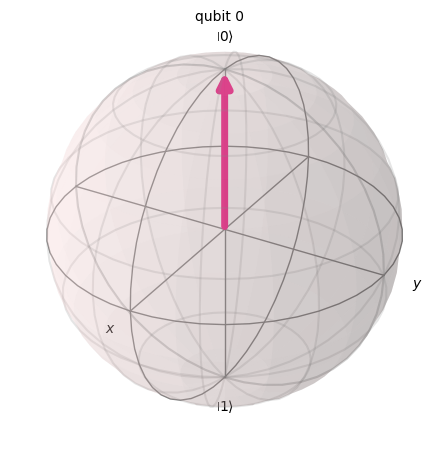
\includegraphics[width=0.5\textwidth]{figures/basis-zustand-blochsphaer.png}
    \caption{Bloch-Sphäre im Basiszustand}
    \label{fig:bloch-basis}
\end{figure}

Der Winkel $\theta$ bestimmt dabei das Verhältnis der beiden Amplituden, der Winkel $\varphi$ ihre relative Phase. Die beiden Basiszustände $\ket{0}$ und $\ket{1}$ liegen am Nord- beziehungsweise Südpol der Kugel, während alle übrigen Punkte der Oberfläche Superpositionen entsprechen. Operationen auf einem Qubit lassen sich in dieser Darstellung als Drehungen des Zustandsvektors um die Achsen der Kugel auffassen. Die Bloch-Sphäre eignet sich damit vor allem zur Veranschaulichung einzelner Qubits.

\newpage
\section{Quantenschaltkreise und Gatter}
\label{sec:gatesCircuits}

Quantenschaltkreise, auch \textit{Circuits} genannt, sind die übliche Darstellungsform für Quantenprogramme im Gattermodell, das auf David Deutsch~\cite{deutsch1985quantum} zurückgeht und heute den Standard für die Programmierung von Quantencomputern bildet. Jedes Qubit erhält seine eigene horizontale Linie, beginnend mit $q_0$.Bei $n$ Qubits hat man daher $n$ Linien, die von $q_0$ bis $q_{n-1}$
nummeriert sind (siehe Abbildung~\ref{fig:circuit-cnot}).. Auf diese Linien werden von links nach rechts \textit{Quantengatter} angewendet, die die Zustände der Qubits manipulieren~\cite{nielsen2010chuang,homeister2022quantum}.
Am Ende eines Circuits steht in der Regel eine \textit{Messung}, die den Quantenzustand auf einen klassischen Bitwert reduziert und pro Qubit den Wert $0$ oder $1$ liefert. Da das Ergebnis einer einzelnen Messung zufällig ist, lässt sich aus einem einzigen Durchlauf noch keine Aussage über den zugrundeliegenden Zustand ableiten. Erst die vielfache Ausführung desselben Circuits liefert eine Verteilung der Ergebnisse, aus der sich die Wahrscheinlichkeiten der möglichen Messwerte abschätzen lassen. Die Anzahl dieser Wiederholungen wird als \textit{Shots} bezeichnet~\cite{nielsen2010chuang,bashiri2025quantencomputing}.

Es gibt verschiedene Arten von Gattern. Einqubit-Gatter lassen sich als $2 \times 2$-Matrix darstellen. Jedoch gibt es auch Gatter, die auf mehrere Qubits wirken. Ein Gatter, das auf $n$ Qubits wirkt, entspricht einer unitären $2^{n} \times 2^{n}$-Matrix.
\newpage

\paragraph*{X-Gatter}\mbox{}\\
Das \textit{X-Gatter} stellt das quantenmechanische Analogon der klassischen
NOT-Operation dar und vertauscht die Amplituden der Basiszustände $\ket{0}$ und
$\ket{1}$. Seine Matrixdarstellung lautet
\begin{equation}
    \mathbf{X} = \begin{pmatrix} 0 & 1 \\ 1 & 0 \end{pmatrix}.
\end{equation}
Angewendet auf den Ausgangszustand $\ket{0}$ ergibt sich
\begin{equation}
    \mathbf{X}\ket{0}
    = \begin{pmatrix} 0 & 1 \\ 1 & 0 \end{pmatrix}
      \begin{pmatrix} 1 \\ 0 \end{pmatrix}
    = \begin{pmatrix} 0 \\ 1 \end{pmatrix}
    = \ket{1}.
\end{equation}
Der Zustand wird somit deterministisch in $\ket{1}$ überführt, es gilt also
$p(0) = 0$ und $p(1) = 1$. Eine Superposition entsteht dabei nicht. Auf der
Bloch-Sphäre entspricht das X-Gatter einer Drehung um $\pi$ um die $x$-Achse,
wodurch der Zustandsvektor vom Nordpol zum Südpol wandert (siehe
Abbildung~\ref{fig:x-gatter}).

\begin{figure}[htbp]
    \centering
    \begin{subfigure}{0.45\textwidth}
        \centering
        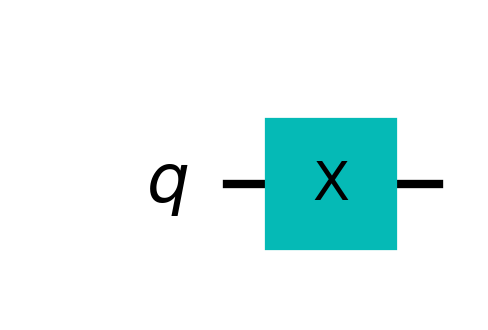
\includegraphics[width=0.65\linewidth]{figures/DarstellungGatter/x_gatter_circuit.png}
        \subcaption{Schaltkreis mit \textit{X}-Gatter}
        \label{fig:circuit-x}
    \end{subfigure}\hfill
    \begin{subfigure}{0.45\textwidth}
        \centering
        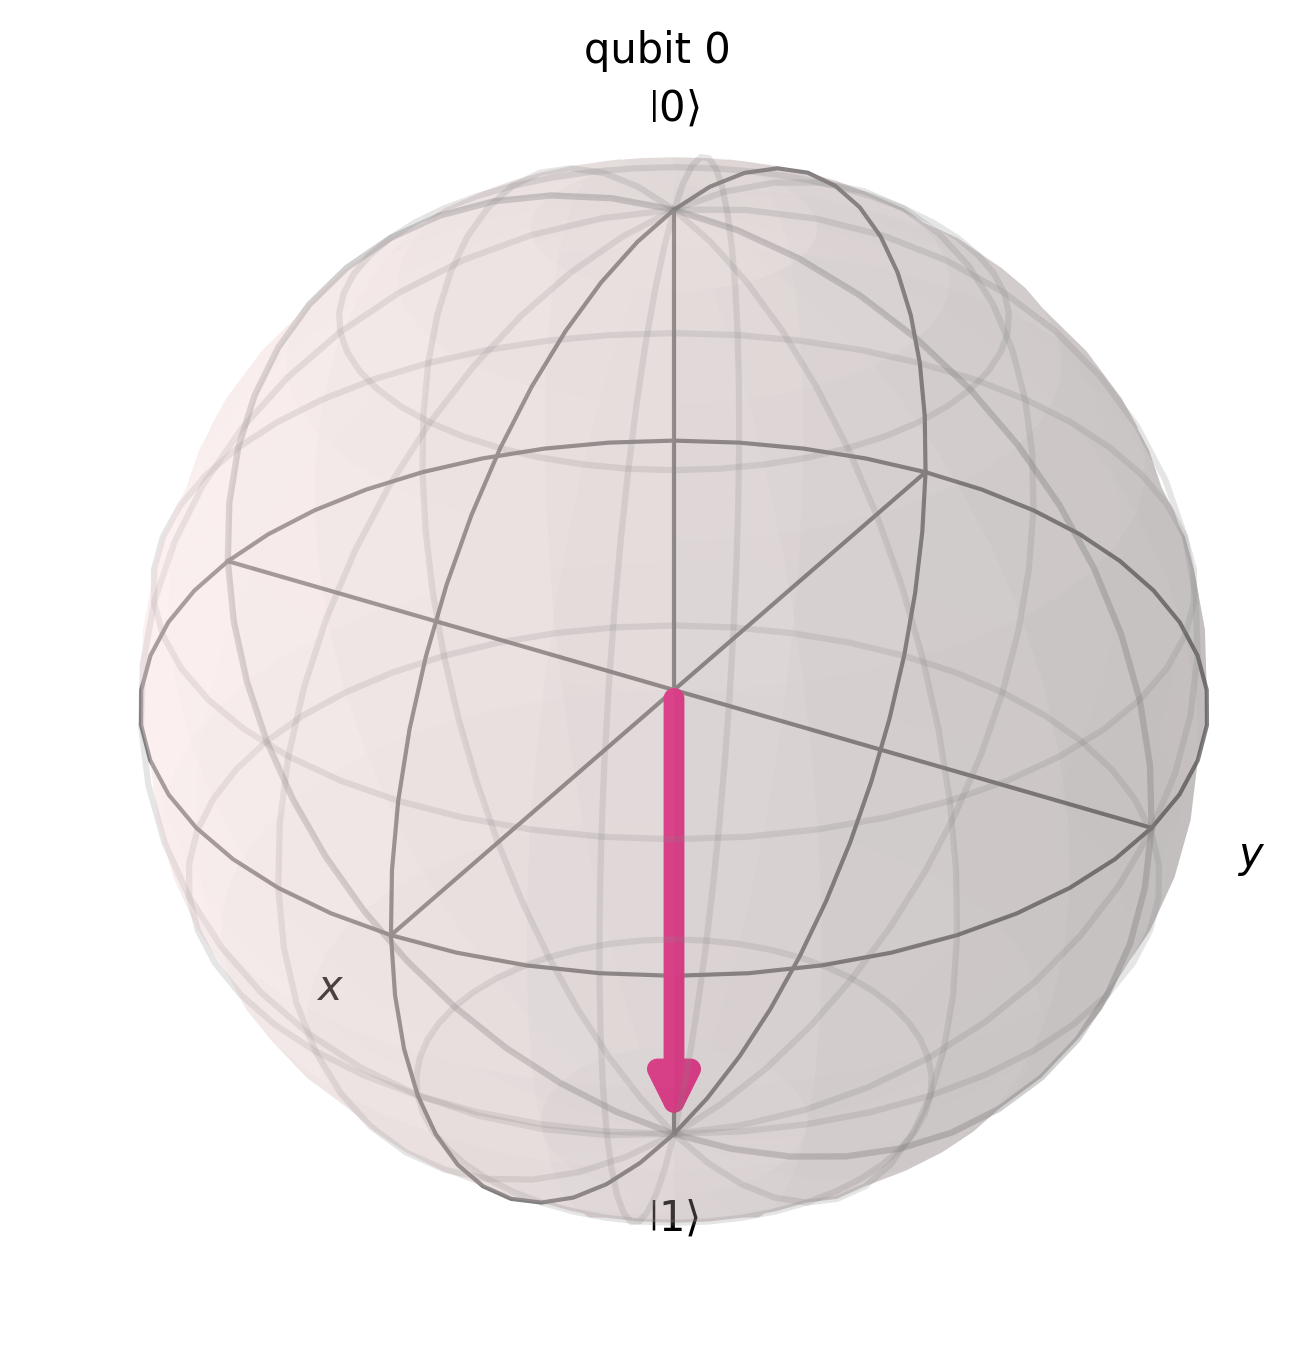
\includegraphics[width=0.65\linewidth]{figures/DarstellungGatter/x_gatter_bloch.png}
        \subcaption{Zustand auf der Bloch-Sphäre}
        \label{fig:bloch-x}
    \end{subfigure}
    \caption{Wirkung des \textit{X}-Gatters}
    \label{fig:x-gatter}
\end{figure}

\paragraph*{Hadamard-Gatter}\mbox{}\\
Das \textit{Hadamard-Gatter} erzeugt aus einem Basiszustand eine gleichgewichtete
Superposition und realisiert damit den Basiswechsel zwischen der $Z$- und der
$X$-Basis. Es besitzt die Matrixdarstellung
\begin{equation}
    \mathbf{H} = \frac{1}{\sqrt{2}}
    \begin{pmatrix} 1 & 1 \\ 1 & -1 \end{pmatrix}.
\end{equation}
Die Anwendung auf den Ausgangszustand $\ket{0}$ liefert
\begin{equation}
    \mathbf{H}\ket{0}
    = \frac{1}{\sqrt{2}}
      \begin{pmatrix} 1 & 1 \\ 1 & -1 \end{pmatrix}
      \begin{pmatrix} 1 \\ 0 \end{pmatrix}
    = \frac{1}{\sqrt{2}}
      \begin{pmatrix} 1 \\ 1 \end{pmatrix}
    = \frac{1}{\sqrt{2}}\bigl(\ket{0} + \ket{1}\bigr).
\end{equation}
Beide Messergebnisse treten folglich mit gleicher Wahrscheinlichkeit
$p(0) = p(1) = \tfrac{1}{2}$ auf, wie in Abbildung~\ref{fig:h-gatter} dargestellt.
Da $\mathbf{H}^2 = \mathbf{I}$ gilt, ist das Hadamard-Gatter zugleich sein eigenes
Inverses.

\begin{figure}[htbp]
    \centering
    \begin{subfigure}{0.45\textwidth}
        \centering
        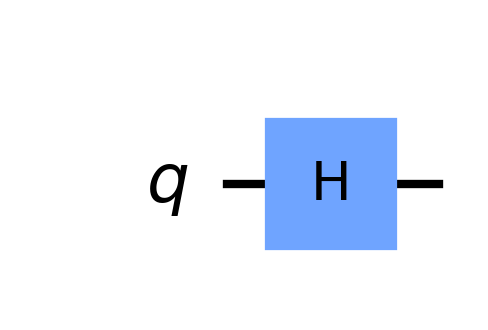
\includegraphics[width=0.65\linewidth]{figures/DarstellungGatter/h_gatter_circuit.png}
        \subcaption{Schaltkreis mit \textit{H}-Gatter}
        \label{fig:circuit-h}
    \end{subfigure}\hfill
    \begin{subfigure}{0.45\textwidth}
        \centering
        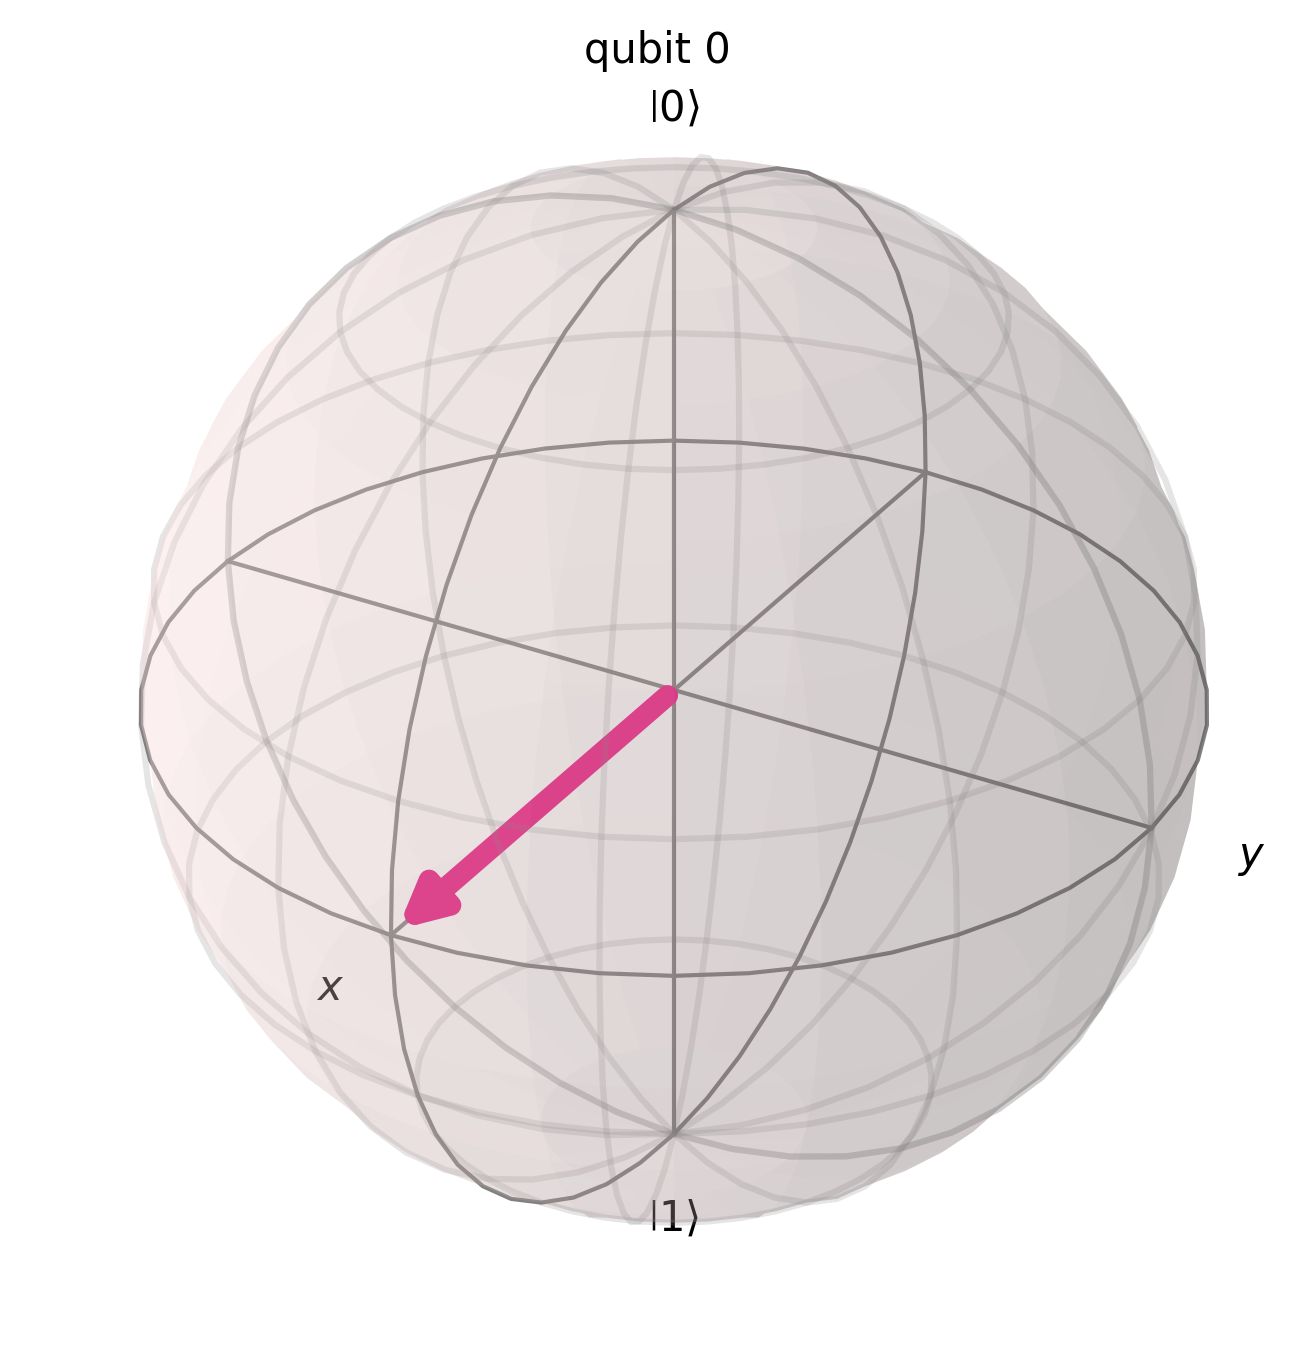
\includegraphics[width=0.65\linewidth]{figures/DarstellungGatter/h_gatter_bloch.png}
        \subcaption{Zustand auf der Bloch-Sphäre}
        \label{fig:bloch-h}
    \end{subfigure}
    \caption{Wirkung des Hadamard-Gatters}
    \label{fig:h-gatter}
\end{figure}

\paragraph*{T-Gatter}\mbox{}\\
Das \textit{T-Gatter} gehört zur Klasse der Phasengatter. Es lässt den Basiszustand
$\ket{0}$ unverändert und prägt dem Zustand $\ket{1}$ eine relative Phase von
$e^{i\pi/4}$ auf. Seine Matrixdarstellung lautet
\begin{equation}
    \mathbf{T} = \begin{pmatrix} 1 & 0 \\ 0 & e^{i\pi/4} \end{pmatrix}.
\end{equation}
Angewendet auf einen allgemeinen Zustand
$\ket{\psi} = \alpha\ket{0} + \beta\ket{1}$ ergibt sich
\begin{equation}
    \mathbf{T}\ket{\psi} = \alpha\ket{0} + e^{i\pi/4}\beta\ket{1}.
\end{equation}
Da die Phase den Betrag der Amplituden nicht verändert, bleiben die
Messwahrscheinlichkeiten in der Rechenbasis unbeeinflusst. Die aufgeprägte
Phaseninformation wird erst durch nachfolgende Gatter beobachtbar, die einen
Basiswechsel bewirken.

Auf den Zustand $\ket{0}$ angewendet, bleibt das T-Gatter ohne Wirkung, da die Phase
allein den Anteil $\ket{1}$ betrifft. Um die Phase überhaupt sichtbar zu machen,
wird dem T-Gatter daher ein Hadamard-Gatter vorangestellt. Dieses erzeugt zunächst
eine gleichgewichtete Superposition, sodass beide Basiszustände am Gesamtzustand
beteiligt sind. Erst dann verschiebt das T-Gatter den Zustandsvektor auf der
Bloch-Sphäre entlang des Äquators um $45$ Grad, wie in
Abbildung~\ref{fig:h-t-gatter} dargestellt. Die Messwahrscheinlichkeiten bleiben
dabei weiterhin bei $p(0) = p(1) = \tfrac{1}{2}$.

\begin{figure}[htbp]
    \centering
    \begin{subfigure}{0.45\textwidth}
        \centering
        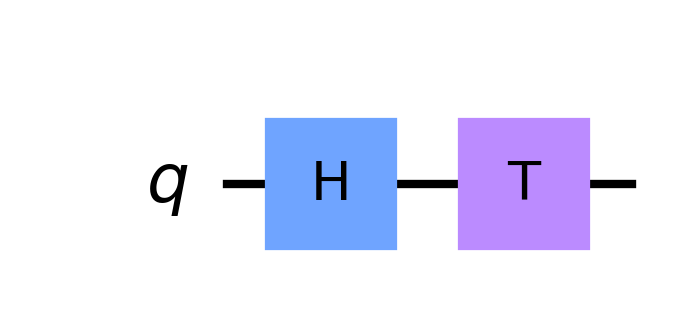
\includegraphics[width=0.65\linewidth]{figures/DarstellungGatter/h_t_gatter_circuit.png}
        \subcaption{Schaltkreis mit \textit{H}- und \textit{T}-Gatter}
        \label{fig:circuit-h-t}
    \end{subfigure}\hfill
    \begin{subfigure}{0.45\textwidth}
        \centering
        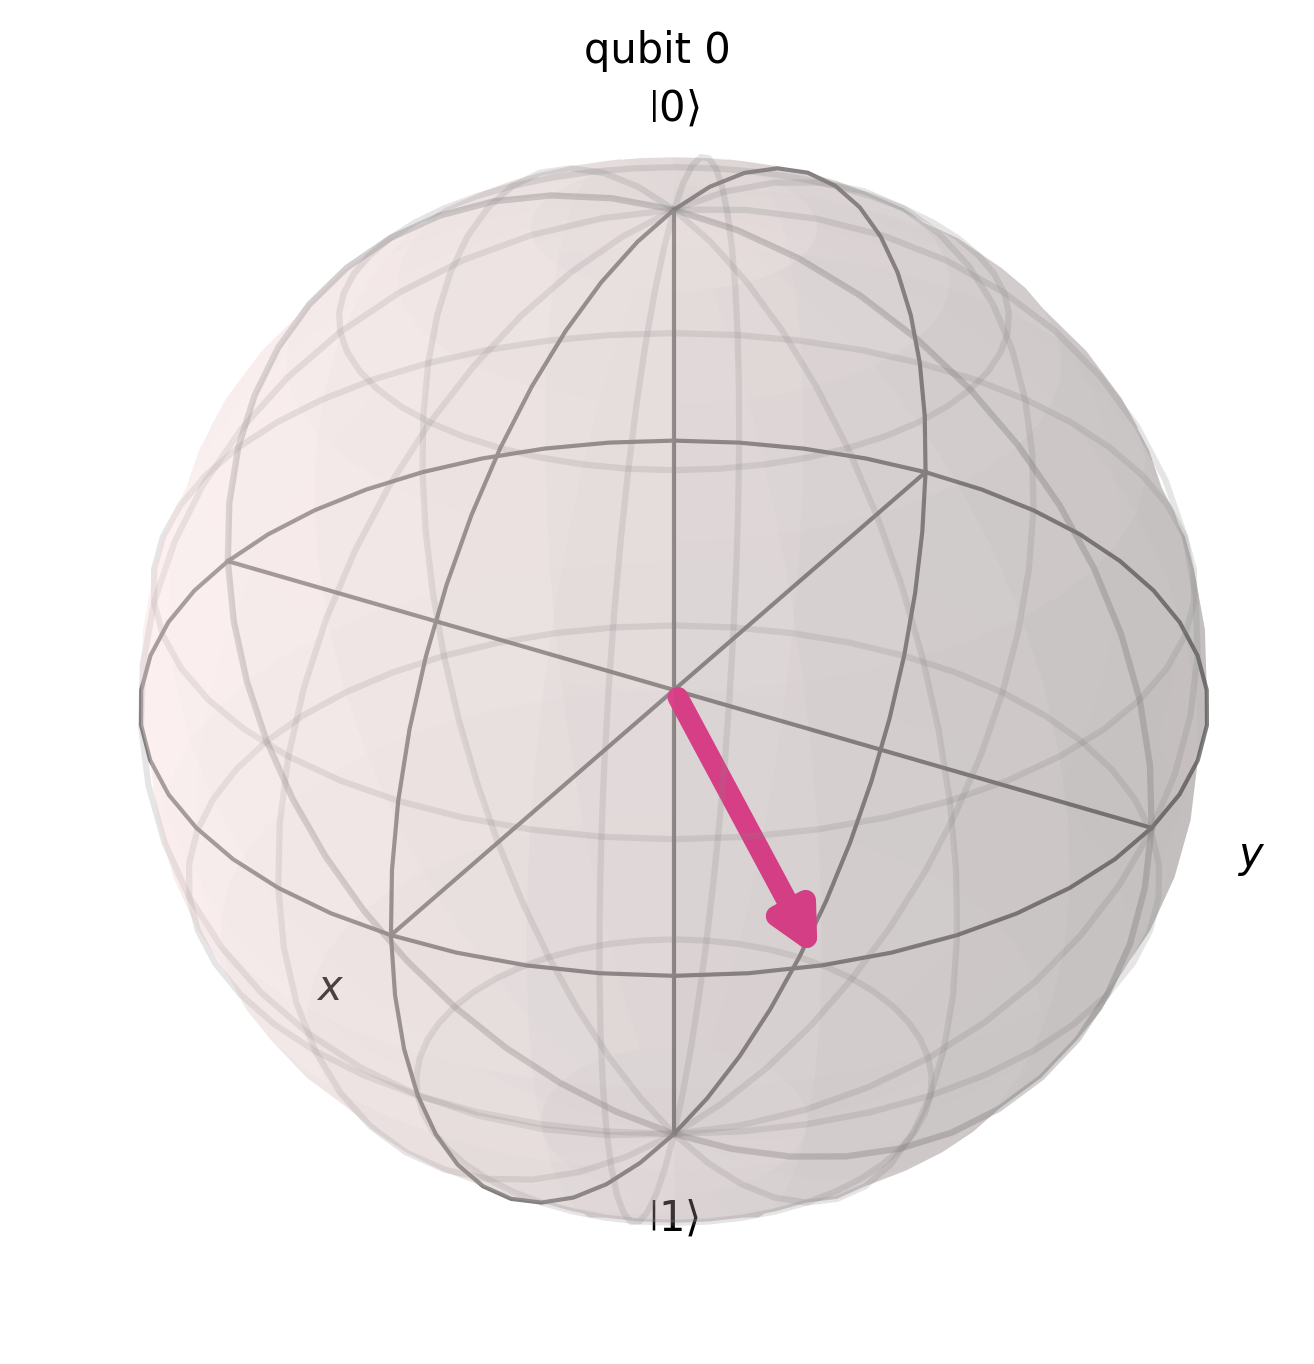
\includegraphics[width=0.65\linewidth]{figures/DarstellungGatter/h_t_gatter_bloch.png}
        \subcaption{Zustand auf der Bloch-Sphäre}
        \label{fig:bloch-h-t}
    \end{subfigure}
    \caption{Sichtbarwerden der Phase durch ein vorgeschaltetes Hadamard-Gatter}
    \label{fig:h-t-gatter}
\end{figure}

\newpage

\paragraph*{RY-Gatter}\mbox{}\\
Das \textit{RY-Gatter} gehört zur Klasse der Rotationsgatter und beschreibt eine
Drehung des Qubitzustands um die $y$-Achse der Bloch-Sphäre um einen frei
wählbaren Winkel $\theta$. Seine Matrixdarstellung lautet
\begin{equation}
    \mathbf{R}_y(\theta) =
    \begin{pmatrix}
        \cos\frac{\theta}{2} & -\sin\frac{\theta}{2} \\[2pt]
        \sin\frac{\theta}{2} & \cos\frac{\theta}{2}
    \end{pmatrix}.
\end{equation}
Angewendet auf den Ausgangszustand $\ket{0}$ ergibt sich
\begin{equation}
    \mathbf{R}_y(\theta)\ket{0}
    = \begin{pmatrix}
        \cos\frac{\theta}{2} & -\sin\frac{\theta}{2} \\[2pt]
        \sin\frac{\theta}{2} & \cos\frac{\theta}{2}
      \end{pmatrix}
      \begin{pmatrix} 1 \\ 0 \end{pmatrix}
    = \cos\tfrac{\theta}{2}\ket{0} + \sin\tfrac{\theta}{2}\ket{1}.
\end{equation}
Der Winkel $\theta$ legt fest, wie stark sich der Zustand von $\ket{0}$ entfernt.
Die Messwahrscheinlichkeiten betragen $p(0) = \cos^2\tfrac{\theta}{2}$ und
$p(1) = \sin^2\tfrac{\theta}{2}$. Bei $\theta = 0$ bleibt $\ket{0}$ erhalten, bei
$\theta = \pi$ entsteht $\ket{1}$. Dazwischen liegt eine Superposition beider
Zustände. Für $\theta = \tfrac{\pi}{2}$ ergibt sich beispielsweise
\begin{equation}
    \mathbf{R}_y\!\left(\tfrac{\pi}{2}\right)\ket{0}
    = \frac{1}{\sqrt{2}}\bigl(\ket{0} + \ket{1}\bigr),
\end{equation}
also eine gleichgewichtete Superposition mit $p(0) = p(1) = \tfrac{1}{2}$, wie sie
auch das Hadamard-Gatter aus $\ket{0}$ erzeugt (siehe
Abbildung~\ref{fig:ry-gatter}). Alle Einträge der Matrix sind reell, weshalb sich
das RY-Gatter gut eignet, um klassische Daten in den Amplituden abzubilden.

Für beliebige Werte von $\theta$ gehört das RY-Gatter nicht zur Clifford-Gruppe.
Als parametrisiertes Gatter wird es vor allem in variationellen
Quantenschaltkreisen eingesetzt. Damit sind Schaltkreise gemeint, deren Parameter
von einem klassischen Optimierer schrittweise angepasst werden, bis ein
gewünschtes Ergebnis erreicht ist.

\begin{figure}[htbp]
    \centering
    \begin{subfigure}{0.45\textwidth}
        \centering
        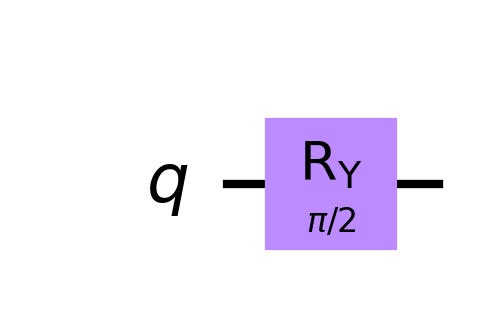
\includegraphics[width=0.65\linewidth]{figures/DarstellungGatter/ry_gatter_circuit.png}
        \subcaption{Schaltkreis mit \textit{RY}-Gatter}
        \label{fig:circuit-ry}
    \end{subfigure}\hfill
    \begin{subfigure}{0.45\textwidth}
        \centering
        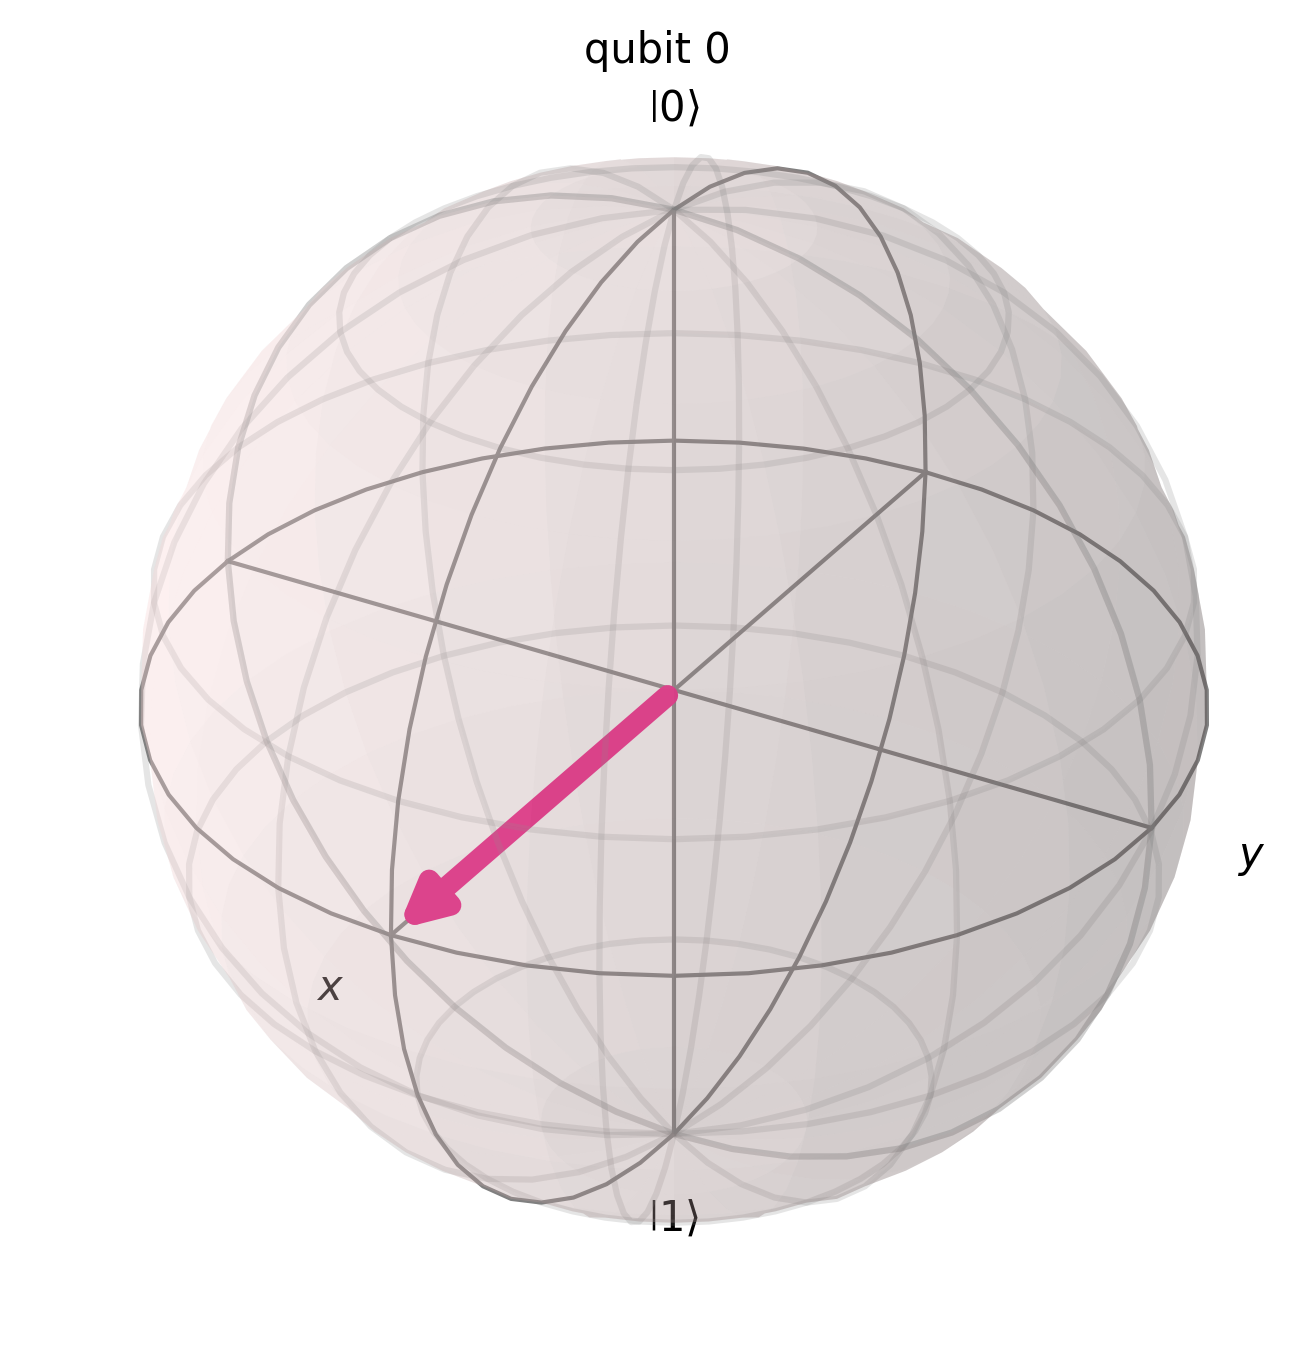
\includegraphics[width=0.65\linewidth]{figures/DarstellungGatter/ry_gatter_bloch.png}
        \subcaption{Zustand auf der Bloch-Sphäre}
        \label{fig:bloch-ry}
    \end{subfigure}
    \caption{Wirkung des \textit{RY}-Gatters für $\theta = \tfrac{\pi}{2}$}
    \label{fig:ry-gatter}
\end{figure}

\paragraph*{CNOT-Gatter}\mbox{}\\
Das \textit{CNOT-Gatter} (auch \textit{CX-Gatter}) ist das wichtigste
Zweiqubit-Gatter. Es wirkt auf ein \textit{Kontrollqubit} und ein
\textit{Zielqubit}. Befindet sich das Kontrollqubit im Zustand $\ket{1}$, wird auf
das Zielqubit eine $\mathbf{X}$-Operation angewendet, andernfalls bleibt das
Zielqubit unverändert. In der Zweiqubit-Basis
$\{\ket{00}, \ket{01}, \ket{10}, \ket{11}\}$ lautet die Matrixdarstellung
\begin{equation}
    \mathbf{CX} =
    \begin{pmatrix}
        1 & 0 & 0 & 0 \\
        0 & 1 & 0 & 0 \\
        0 & 0 & 0 & 1 \\
        0 & 0 & 1 & 0
    \end{pmatrix}.
\end{equation}
Die Wirkung auf die Basiszustände ergibt sich entsprechend zu
\begin{equation}
    \mathbf{CX}\ket{00} = \ket{00}, \quad
    \mathbf{CX}\ket{01} = \ket{01}, \quad
    \mathbf{CX}\ket{10} = \ket{11}, \quad
    \mathbf{CX}\ket{11} = \ket{10}.
\end{equation}
Wird das Gatter auf einen Basiszustand angewendet, entsteht dabei stets wieder ein
Produktzustand. Die besondere Bedeutung des CNOT-Gatters liegt darin, dass es aus einer
Superposition des Kontrollqubits Verschränkung erzeugt.
\begin{equation}
    \mathbf{CX}_{12}\,\mathbf{H}_1\ket{00}
    = \mathbf{CX}_{12}\,\frac{1}{\sqrt{2}}\bigl(\ket{00} + \ket{10}\bigr)
    = \frac{1}{\sqrt{2}}\bigl(\ket{00} + \ket{11}\bigr).
\end{equation}
Das Hadamard-Gatter versetzt zunächst das erste Qubit in eine Superposition (siehe
Abbildung~\ref{fig:circuit-cnot}). Das CNOT-Gatter wirkt anschließend auf beide
Anteile zugleich. Der Anteil $\ket{00}$ bleibt unverändert, im Anteil $\ket{10}$
wird das Zielqubit umgeklappt. Im Ergebnis liefern beide Qubits bei einer Messung
stets dasselbe Resultat, und der Zustand lässt sich nicht mehr als Tensorprodukt
einzelner Qubitzustände schreiben.

Anders als bei den bisher betrachteten Gattern lässt sich das Ergebnis nicht mehr
auf der Bloch-Sphäre darstellen. Diese beschreibt jeweils den Zustand eines
einzelnen Qubits, ein verschränkter Zustand ist jedoch nur als Ganzes definiert.
Betrachtet man eines der beiden Qubits für sich, so liefert es in jeder
Messrichtung beide Ergebnisse mit gleicher Wahrscheinlichkeit. Die eigentliche
Information liegt nicht in den einzelnen Qubits, sondern in ihrer Korrelation und
entzieht sich damit einer getrennten Darstellung.

\begin{figure}[htbp]
    \centering
    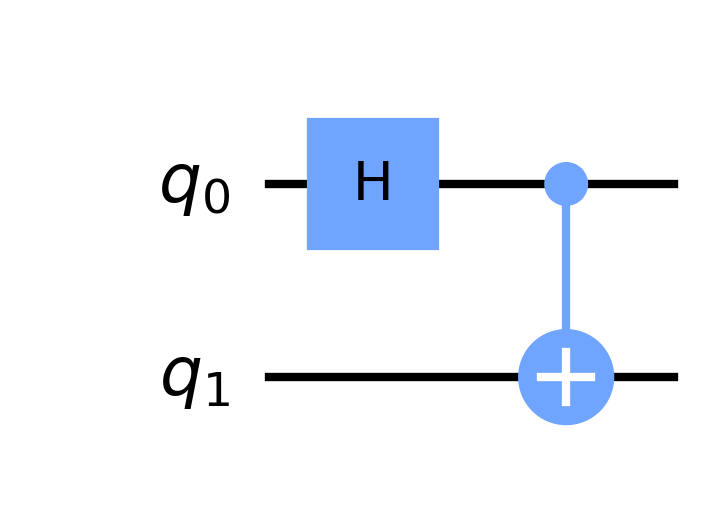
\includegraphics[width=0.3\textwidth]{figures/DarstellungGatter/cnot_gatter_circuit.png}
    \caption{Schaltkreis mit \textit{H}- und \textit{CNOT}-Gatter}
    \label{fig:circuit-cnot}
\end{figure}

% ----------------------------------------------------------------
\newpage

\section{Observablenberechnung}
\label{sec:observablen}

Als \textit{Observable} wird in der Quantenmechanik eine messbare physikalische
Größe bezeichnet, die durch einen hermiteschen Operator repräsentiert
wird~\cite{nielsen2010chuang}. Ein Operator heißt \textit{hermitesch}, wenn er mit
seinem adjungierten Operator übereinstimmt, also $O = O^{\dagger}$ gilt, wobei
$O^{\dagger}$ die konjugiert transponierte Matrix bezeichnet. Diese Eigenschaft
stellt sicher, dass alle Eigenwerte reell sind, was Voraussetzung dafür ist, dass
sie als physikalische Messwerte interpretiert werden können. Welcher Eigenwert bei
einer einzelnen Messung auftritt, ist im Allgemeinen nicht vorhersagbar, sondern
folgt einer durch den Quantenzustand festgelegten Wahrscheinlichkeitsverteilung.

Da einzelne Messungen zufällig ausfallen, ist im Quantencomputing weniger das
Einzelergebnis als vielmehr der \textit{Erwartungswert} einer Observablen $O$
bezüglich eines Zustands $\ket{\psi}$ von Interesse. Dieser ist definiert als
\[
    \expval{O} = \bra{\psi} O \ket{\psi}
\]
und beschreibt den statistischen Mittelwert der Messergebnisse über viele
Wiederholungen. Seine Berechnung beziehungsweise Schätzung bildet die Grundlage zahlreicher
Quantenalgorithmen.

Für die konkrete Darstellung von Observablen werden üblicherweise die
Pauli-Operatoren $I$, $X$, $Y$ und $Z$ herangezogen. Diese bilden mit reellen
Koeffizienten eine Basis des Raums der hermiteschen $2 \times 2$-Matrizen, sodass
sich jede Observable eines einzelnen Qubits als Linearkombination dieser vier
Operatoren schreiben lässt~\cite{nielsen2010chuang}. Für Systeme mehrerer Qubits
werden Observablen entsprechend als Linearkombination von Tensorprodukten dieser
Operatoren ausgedrückt, die als \enquote{Pauli-Strings} bezeichnet werden.
\newpage
\chapter{Quantencomputing-Software}
\label{chap:software}

Im Quantencomputing wird eine Vielzahl von Frameworks eingesetzt, die meist auf dem Konzept von Schaltkreisen und Gattern beruhen. In diesem Abschnitt werden die beiden Frameworks \textit{PennyLane} und \textit{Qiskit} vorgestellt, die später auch in der Implementierung und dem Benchmark genutzt werden. Zudem werden der Executor, in dem die Abstraktionsschicht implementiert wurde, sowie auf dem Markt vorhandene Alternativen vorgestellt.

\section{PennyLane}
\label{sec:pennylane}
\textit{PennyLane} ist ein auf Python basierendes Open-Source-Framework (Apache License 2.0) für Quantencomputing, das von dem kanadischen Quantencomputing-Unternehmen Xanadu entwickelt wurde~\cite{bergholm2018pennylane}. Das zentrale Merkmal des Frameworks ist die Berechnung von Gradienten parametrisierter Quantenschaltkreise~\cite{schuld2019evaluating} auf eine Weise, die mit klassischen Verfahren wie der Backpropagation kompatibel ist~\cite{baydin2018automatic}. Die aus dem maschinellen Lernen bekannten Methoden der automatischen Differentiation werden so auf quantenmechanische und hybride Berechnungen ausgeweitet~\cite{bergholm2018pennylane}. Damit ist \textit{PennyLane} insbesondere auf den Einsatz von maschinellem Lernen mit Quantencomputern ausgelegt.

Von Haus aus liefert \textit{PennyLane} eigene integrierte Simulatoren mit, darunter den Statevector-Simulator \texttt{lightning.qubit}~\cite{bergholm2018pennylane}. Darüber hinaus stehen den Anwenderinnen und Anwendern über zahlreiche Plugins die Backends diverser externer Plattformen zur Verfügung, darunter IBM Quantum (\textit{Qiskit}), Amazon Braket, Google \textit{Cirq} sowie \textit{Qulacs}~\cite{bergholm2018pennylane}. In dieser Arbeit wird \textit{PennyLane} in Version~0.42.3 verwendet.

\newpage
\section{Qiskit}
\label{sec:qiskit}
Das bereits als Plugin-Backend erwähnte \textit{Qiskit} ist ein auf Python basierendes Open-Source-Framework (Apache License 2.0) für Quantencomputing, das von IBM entwickelt und im Jahr 2017 veröffentlicht wurde~\cite{javadiabhari2024quantum}. Im Gegensatz zu \textit{PennyLane}, dessen Architektur primär auf die differenzierbare Programmierung ausgerichtet ist, verfolgt \textit{Qiskit} einen schaltkreiszentrierten Ansatz. Im Mittelpunkt steht die Klasse \texttt{QuantumCircuit}, mit der Quantenschaltkreise auf Gatterebene konstruiert, manipuliert und anschließend ausgeführt werden~\cite{javadiabhari2024quantum}. Ein zentrales Merkmal von \textit{Qiskit} ist der mehrstufige Transpiler, der einen abstrakten Schaltkreis in eine für die Zielhardware ausführbare Form überführt~\cite{javadiabhari2024quantum}.

Für die Simulation stellt das Zusatzpaket \textit{Qiskit Aer} hochperformante, in C++ implementierte Simulatoren bereit, darunter einen Statevector-Simulator sowie Simulatoren auf Basis von Dichtematrizen und des Stabilizer-Formalismus~\cite{javadiabhari2024quantum}. Darüber hinaus ermöglicht \textit{Qiskit} über das Paket \texttt{qiskit-ibm-runtime} den direkten Zugriff auf die Quantenprozessoren der IBM Quantum Platform~\cite{ibmquantum2026runtime,ibmquantum2026docs}. Durch Provider-Pakete von Drittanbietern lassen sich zudem Backends weiterer Hardware-Hersteller ansprechen~\cite{javadiabhari2024quantum}. In dieser Arbeit wird \textit{Qiskit} in Version~2.4.1 verwendet.

\section{Executor}
\label{sec:executor}

Der \textit{Executor} ist eine von Fraunhofer entwickelte Python-Bibliothek, mit der sich Quantenschaltkreise und Observablen über eine einheitliche Abstraktionsschicht definieren und anschließend in einem frei wählbaren Backend ausführen lassen. Die Software baut auf der ebenfalls von Fraunhofer entwickelten \textit{sQUlearn}-Bibliothek auf, die intern ebenfalls einen Executor integriert. Die Grundidee besteht darin, die Beschreibung eines Quantenalgorithmus von der konkreten Software zu trennen, die ihn ausführt. Nutzerinnen und Nutzer formulieren einen Schaltkreis somit nur einmal und können ihn wahlweise etwa mit \textit{Qiskit} oder \textit{PennyLane} berechnen lassen, ohne den Code anpassen zu müssen. Das gewünschte Backend wird lediglich über seinen Namen ausgewählt.

Über diese Schnittstelle stehen die zentralen Operationen des Quantencomputing einheitlich zur Verfügung, insbesondere die Berechnung von Erwartungswerten, das Ziehen von Messproben (Sampling), die Bestimmung des Zustandsvektors sowie von Ableitungen. Die eigentliche Umrechnung in das jeweilige Zielformat übernimmt das Backend automatisch im Hintergrund, sodass sich die Nutzung für verschiedene Frameworks gleich anfühlt. Dadurch verbessert die Bibliothek vor allem die Vergleichbarkeit und Reproduzierbarkeit von Ergebnissen über unterschiedliche Backends hinweg.

In dem Stand vor dieser Arbeit wurde für die Definition von Schaltkreisen und Observablen intern noch ein \textit{Qiskit}-Wrapper verwendet. Die abstrakte Beschreibung stützte sich dabei auf \textit{Qiskit}-Objekte als Zwischenrepräsentation und war somit noch an dieses Framework gebunden. Diese Abhängigkeit widerspricht dem Ziel einer vollständig framework-neutralen Abstraktionsschicht und wird in der Weiterentwicklung durch eine eigenständige, von \textit{Qiskit} unabhängige Darstellung ersetzt. Im Verlauf dieser Arbeit wird gezeigt, wie in dem Executor eine solche Abstraktionsschicht entwickelt und implementiert wurde.
\newpage

% ----------------------------------------------------------------
\section{Stand der Technik}
\label{sec:related_work}

Einen vergleichbaren Ansatz zur \textit{Executor Abstraction} wählt zudem die
\textit{qBraid-SDK}, mit der sich Quantenprogramme beliebiger populärer
Quantenframeworks definieren lassen. Diese werden zunächst über einen
graphbasierten Transpiler in ein vom Ziel-Backend erwartetes Format
übersetzt und anschließend durch eine Kette von \enquote{Passes} geleitet,
die das Programm an die spezifischen Anforderungen der Zielhardware
anpassen. Am Ende wird der Job über den \enquote{qBraid Runtime Service}
an das gewählte Backend übermittelt und dort berechnet. Ergänzend liefert
die SDK Werkzeuge zur Nachbearbeitung und Visualisierung der Ergebnisse.

Im Gegensatz zum \textit{Executor} liegt der Fokus der \textit{qBraid-SDK}
damit primär auf der einheitlichen Anbindung von Cloud-Quantenhardware
und deren Simulatoren verschiedener Anbieter. Zu beachten ist zudem, dass
der von qBraid empfohlene Workflow über den Runtime Service auf ein
credit-basiertes Abrechnungsmodell zurückgreift, das sowohl den
Zugriff auf QPUs als auch auf die verwalteten Cloud-Simulatoren umfasst. 

Der
\textit{Executor} verfolgt hingegen das Ziel, ein einheitliches Interface
für die Ausführung und vergleichende Bewertung verschiedener klassisch
simulierbarer Backends bereitzustellen, um Benchmarking und
Backend-Auswahl innerhalb einer einzigen Abstraktionsschicht zu
ermöglichen. Da diese Backends lokal ausgeführt werden, entstehen für die
Nutzenden keine laufenden Kosten für die Ausführung der Circuits.
%% ============================================================
%%  04_umsetzung.tex
%%  Kapitel 4: Umsetzung / Implementierung
%% ============================================================
\chapter{Umsetzung und Implementierung der Abstraktionsschicht}
\label{chap:umsetzung}

In diesem Kapitel wird aufgezeigt, wie die Abstraktionsschicht aufgebaut und in den Executor integriert wurde. Hierbei wird zudem besprochen, welche Objekte zur Umwandlung genutzt wurden und weshalb.

\section{Ausgangslage}
\label{sec:ausgangslage}

Vor der Integration einer Definitionsschicht der Circuits gab es bereits die Basis der API-Anbindungen. Der damalige Ansatz bestand darin, einen Schaltkreis über \textit{Qiskit}-Objekte zu definieren und anschließend an das Backend zu übergeben. Damit nutzte man jedoch keinen backendunabhängigen Ansatz, sondern lediglich einen Wrapper um \textit{Qiskit}-Objekte. Jeder Schaltkreis war intern ein \texttt{qiskit.QuantumCircuit}, jede Observable eine \texttt{qiskit.SparsePauliOp} und jeder Parameter ein \textit{Qiskit}-\texttt{ParameterVector} oder dessen Element. Wollte man ein anderes Backend als \textit{Qiskit} verwenden, mussten diese \textit{Qiskit}-Objekte zunächst in das jeweilige Backend-Format zurückübersetzt werden. Dadurch war das Programm ineffizient und von \textit{Qiskit} abhängig.

\section{Wahl der internen Objekte}
\label{sec:interne-objekte}

Zunächst musste entschieden werden, in welches Format die Abstraktion die frameworkunabhängigen Objekte später umwandelt.
Bei der Wahl der internen Objekte in \textit{PennyLane} gab es zwei Optionen. In \textit{PennyLane} unterscheidet man zwischen den Objekten \enquote{Quantum Tape} und \enquote{Quantum Node}, um Circuits als Objekt zu erstellen.

Das Quantum Tape ist die unterste Abstraktionsschicht und wird hauptsächlich für die Entwicklung von Erweiterungen für \textit{PennyLane} genutzt, da es einen kleineren Overhead hat. Das Tape zeichnet die angewendeten Gatter als Liste von Operationen auf. Die Parameter der Gatter werden dabei als \textit{PennyLane}-NumPy-Arrays gespeichert. Dies ist ein Wrapper der \textit{NumPy}-Bibliothek, der die Parameter als differenzierbar markiert. Dadurch wird Backpropagation durch den Circuit möglich.
Der Quantum Node ist eine Abstraktion des Quantum Tapes und die übliche Weise, einen Circuit zu erstellen. Dieses Objekt lässt sich durch den Python-Decorator \texttt{@qml.qnode} erstellen. Intern wird beim Aufruf des QNodes ein Tape erstellt und anschließend auf dem Device ausgeführt. Im Gegensatz zum Tape bietet der QNode mehrere Konfigurationsmöglichkeiten. Eine der wichtigsten hierbei ist die Option \texttt{diff\_method="best"}, um eine alternative Differenzierungsmethode zu Parameter-Shift nutzen zu können. Funktional spricht dies für den QNode, hinsichtlich der Laufzeit war jedoch ein Vorteil der Tapes zu erwarten.

Um die beiden Objekte gegenüberzustellen, wurden zwei Vergleichsebenen
betrachtet. Auf der ersten Ebene wurden Tape und QNode mit derselben
Differenzierungsmethode (Parameter-Shift) betrieben. Damit lässt sich der
reine Overhead isolieren, der durch die zusätzliche Abstraktionsschicht des QNodes entsteht, unabhängig davon, wie der Gradient berechnet wird. Auf
der zweiten Ebene wurde der QNode zusätzlich mit der Option
\texttt{diff\_method="best"} gemessen. In diesem Modus wählt
\textit{PennyLane} auf dem Simulator \texttt{default.qubit} automatisch
Backpropagation, die im Gegensatz zur Parameter-Shift-Regel nicht linear
mit der Anzahl trainierbarer Parameter skaliert~\cite{mitarai2018,schuld2019}.
Dieser Messpunkt bildet damit den Vorteil ab, den der QNode im
praktischen Einsatz bietet, nämlich den Zugriff auf effizientere
Differenzierungsmethoden ohne manuelle Implementierung der zugehörigen
Ausführungslogik.

Die Messungen wurden für Circuits mit 5, 8, 10 und 12 Qubits durchgeführt
und decken jeweils die Phasen Circuit-Erstellung, Ausführung und
Gradientenberechnung bei 10\,000 Gattern und 4 Iterationen ab. Bei der
Gradientenberechnung besitzen 30\,\% der Gatter trainierbare Parameter, die
über den Schaltkreis verteilt wurden. Die Ergebnisse sind in
Abbildung~\ref{fig:alle_time} dargestellt.

\begin{figure}[H]
    \centering
    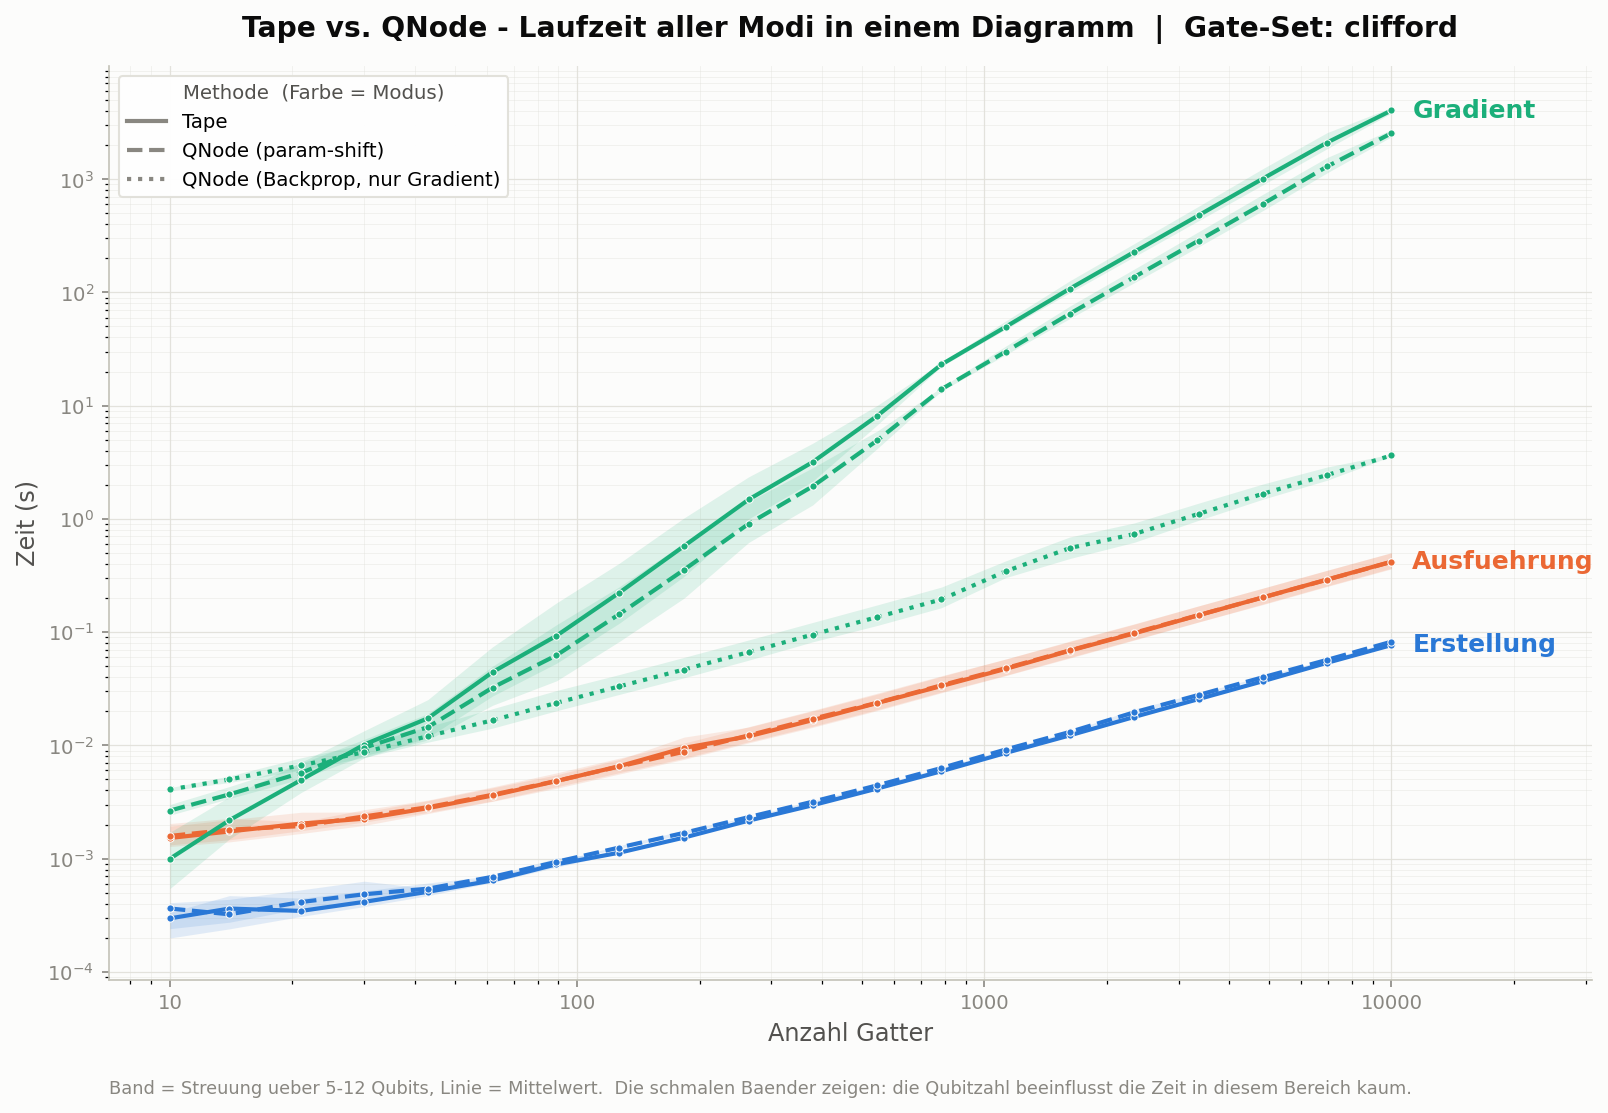
\includegraphics[width=1.0\textwidth]{figures/QnodevsTape/alle_modi_ein_diagramm_time.png}
    \caption{Laufzeiten von Tape und QNode für Erstellung,
  Ausführung und Gradientenberechnung als Mittelwert von 5, 8, 10 und 12 Qubits}
    \label{fig:alle_time}
\end{figure}

Es lässt sich erkennen, dass sowohl bei der Erstellung als auch bei der Ausführung und der Gradientenberechnung mittels Parameter-Shift kaum ein Unterschied zwischen den Tapes und den QNodes besteht. Zudem zeigt sich, dass die QNodes bei der Gradientenberechnung mit
Backpropagation bei 10\,000 Gattern einen Geschwindigkeitsvorteil von rund
36\,\% bis 38\,\% gegenüber den rohen Tapes haben. Parameter-Shift ist allgemein
deutlich langsamer als die \textit{best}-Methode (Backpropagation), da Parameter-Shift zwei
Schaltkreis-Auswertungen pro trainierbarem Parameter benötigt (bei einer Anzahl von 3000 trainierbaren Gattern also $\approx 2 \cdot 3000 = 6000$
Auswertungen), während Backpropagation den vollständigen Gradienten in einem
einzigen Vor- und Rückwärtslauf unabhängig von der Parameterzahl berechnet.
Damit skaliert Parameter-Shift näherungsweise mit
$\mathcal{O}(\text{Gatter}^2)$, Backpropagation dagegen mit
$\mathcal{O}(\text{Gatter})$.

Ein weiteres wichtiges Argument für den QNode war, dass die Parameter der Gatter im Tape nur als feste Werte vorliegen und sich nicht als mathematische Ausdrücke angeben lassen. Da der QNode über eine Python-Funktion definiert wird, gehen die Parameter dort als Argumente ein und können in mathematischen Ausdrücken verwendet werden, bevor sie auf die Gatter angewendet werden. Das passende Tape entsteht daraus erst mit konkreten Werten.

Anders als in \textit{PennyLane} gibt es in \textit{Qiskit} nur ein Circuit-Objekt, den \texttt{QuantumCircuit}. Dieser entspricht dem Tape und war damit die einzige Wahl als internes Zielformat. Ein Gegenstück zum QNode gibt es nicht. Die Gradienten werden stattdessen über separate Parameter-Shift-Klassen aus \texttt{qiskit\_algorithms.gradients} berechnet~\cite{schuld2019}.
\newpage
\section{Implementierung der Abstraktion}
\label{sec:implementierung-abstraktion}

\begin{figure}[H]
    \centering
    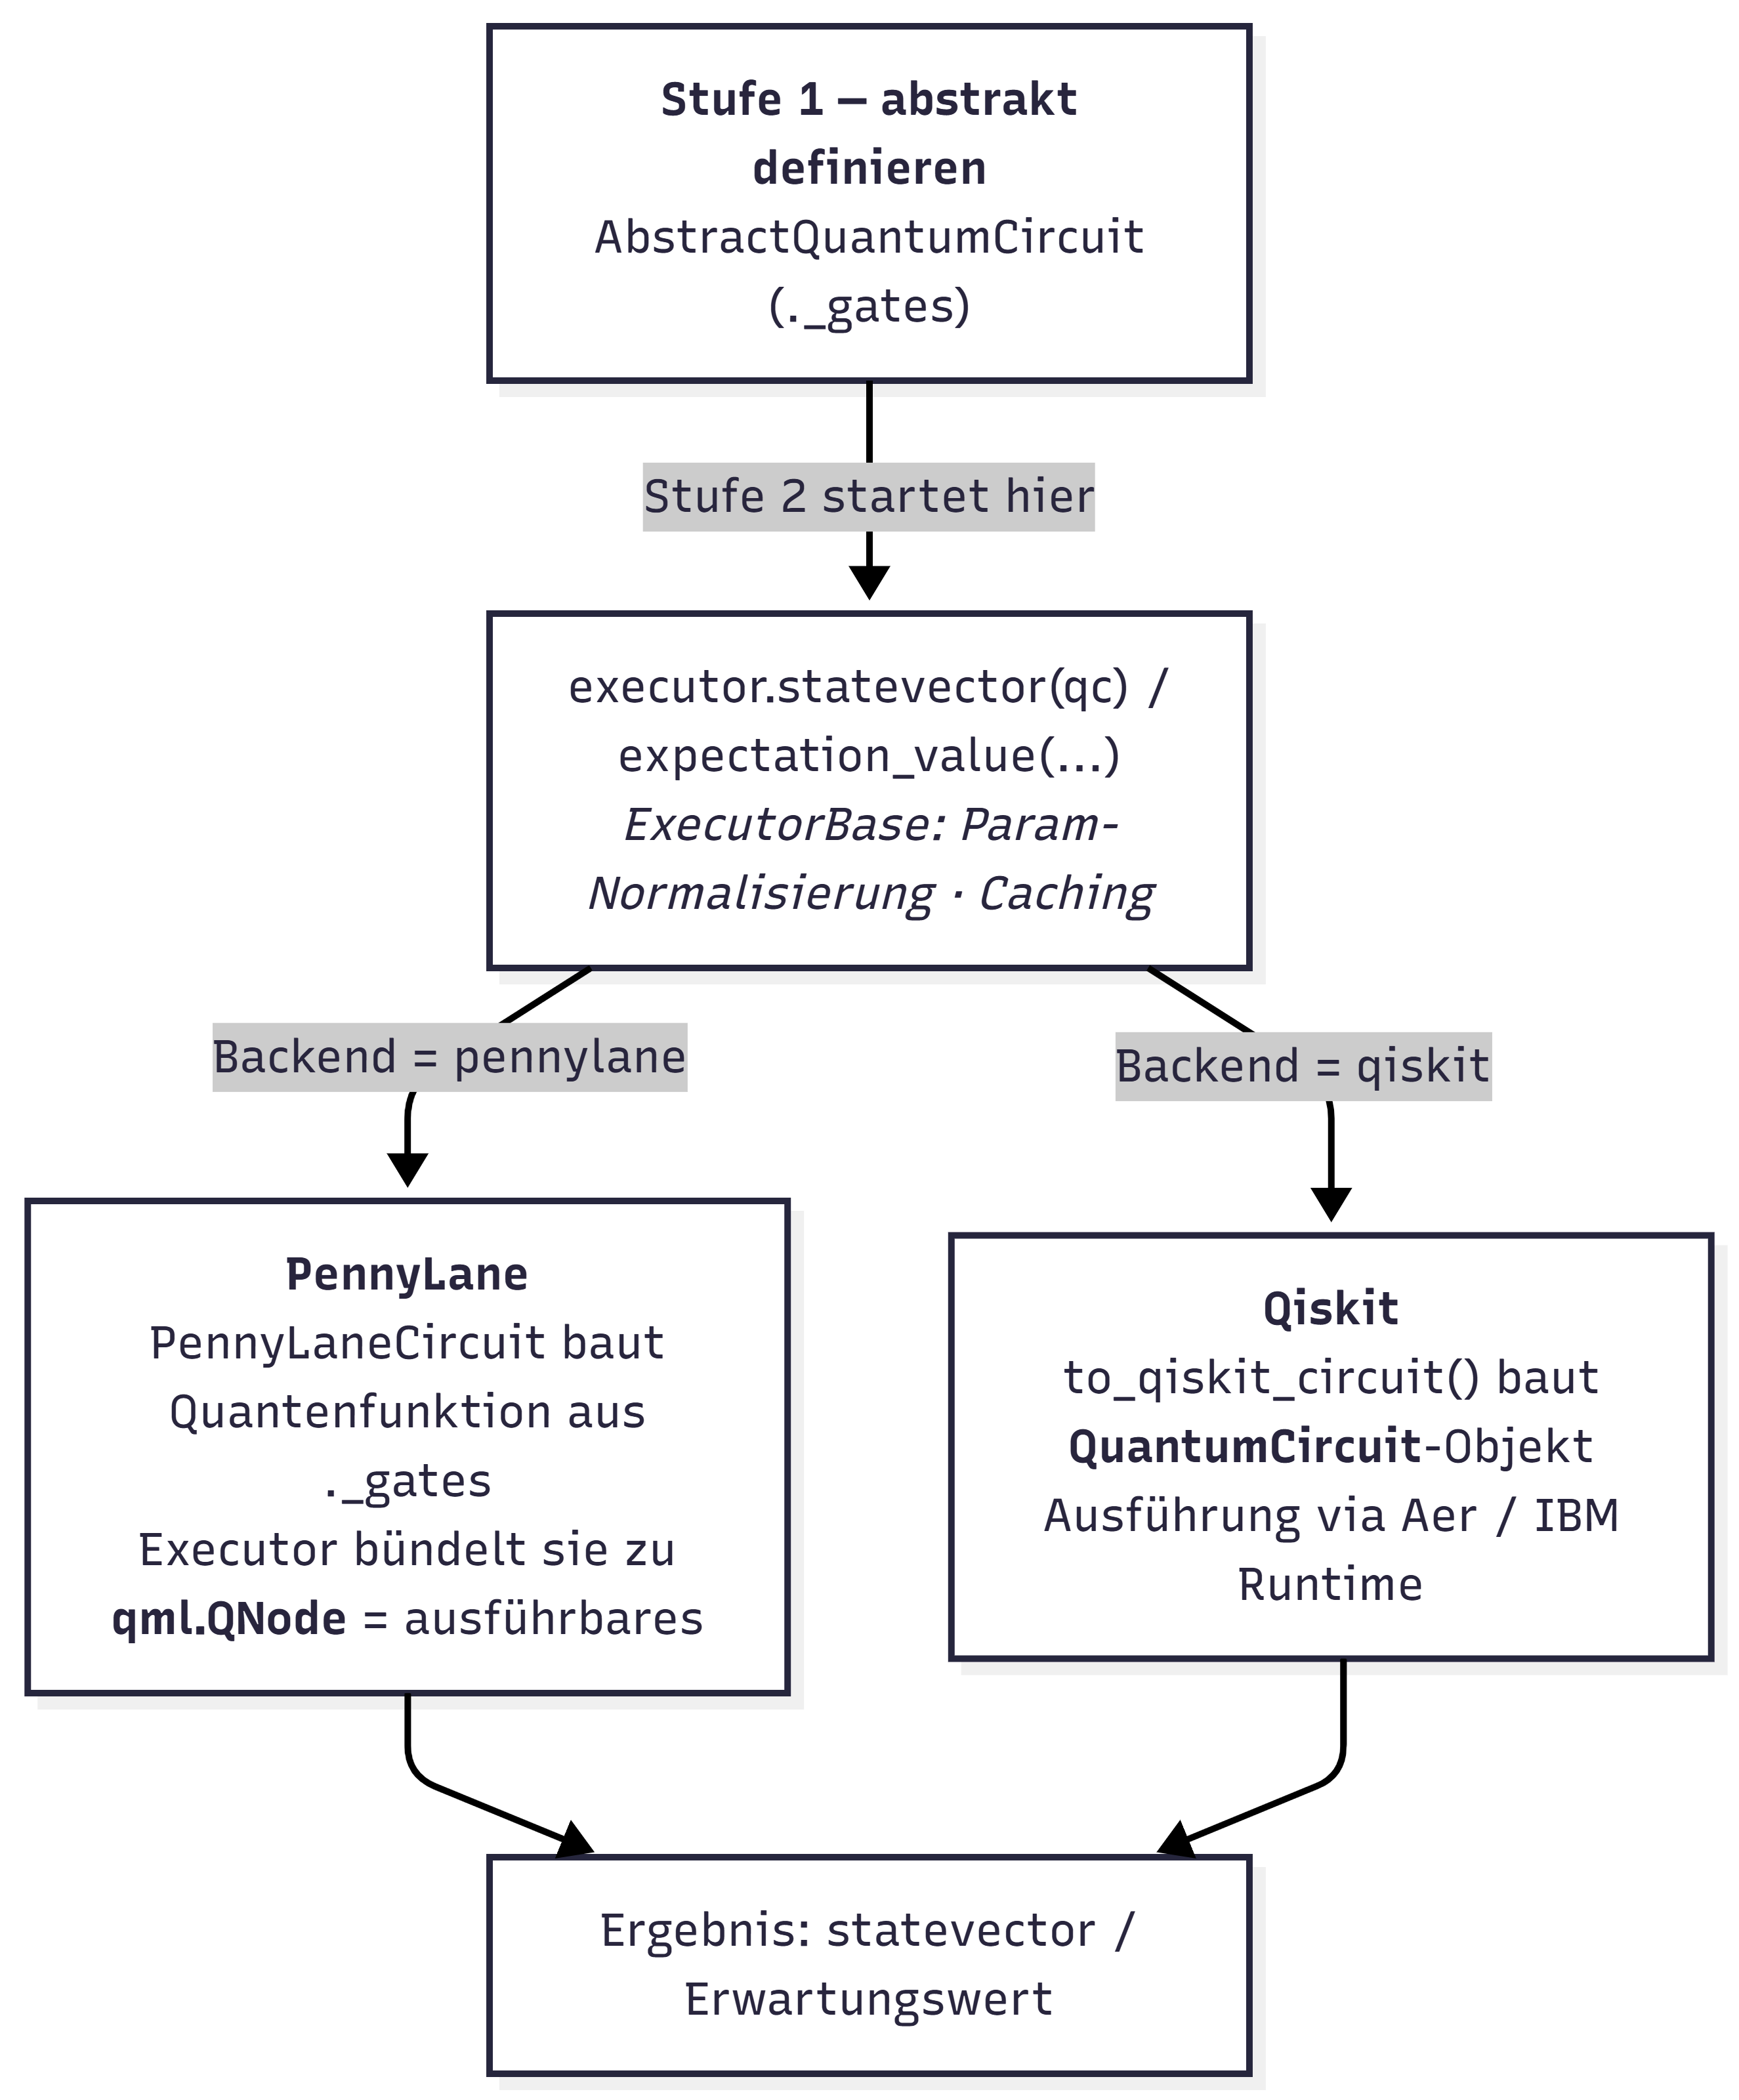
\includegraphics[width=0.6\textwidth]{figures/abstraction-architektur.png}
    \caption{Architektur der Abstraktion}
    \label{fig:abstraktion_architektur}
\end{figure}

Grundlage der Abstraktionsschicht ist eine Datenstruktur, mit der sich ein
Schaltkreis und Observablen über eine eigene, vom Framework unabhängige Syntax beschreiben
lassen. Die wesentliche Schwierigkeit bestand darin, den gemeinsamen
Funktionsumfang der unterstützten Frameworks zu ermitteln, da nur solche
Konstrukte in die Abstraktion aufgenommen werden können, die sich in jedem
Ziel-Backend nachbilden lassen.

Die Abstraktionsschicht ruht auf vier Datentypen, aus denen jedes Backend
anschließend seine eigenen, nativen Objekte erzeugt. Entscheidend ist, dass
diese vier Typen frameworkunabhängig sind. Sie beschreiben, \textit{was}
ausgeführt und gemessen werden soll, treffen jedoch keinerlei Annahmen über das
ausführende Framework und importieren insbesondere keines davon. Damit wird die
im Konzept geforderte Trennung von Definition und Ausführung
(Abschnitt~\ref{sec:konzept-loesung}) auf der Ebene der Datentypen konkret. Die
Nutzerinnen und Nutzer definieren ihren Schaltkreis einmalig in dieser abstrakten Form, während die Übersetzung in ein konkretes Framework erst später und lokal im jeweiligen Backend erfolgt. Hierbei lässt sich das Framework durch das Ändern einer einzigen Variablen wechseln.

\paragraph*{Der Schaltkreis}\mbox{}\\
\label{par:datentypen-schaltkreis}
Ein Schaltkreis wird framework-unabhängig als geordnete Liste typisierter
Gate-Objekte gehalten. Die Reihenfolge der Listenelemente bestimmt die
Ausführungsreihenfolge. Aus dieser Repräsentation ergeben sich zwei
Eigenschaften. Zum einen stellen alle Schaltkreis-Operationen wie das Verketten,
Invertieren, Kopieren und das Binden von Parametern Umformungen dieser Liste dar
und erfordern keinen Aufruf einer Framework-Funktion. Zum anderen gelangt jedes
Gatter über eine einzige Stelle in die Liste, an der die Validierung erfolgt.
Geprüft werden die Zugehörigkeit zum gemeinsamen Vokabular, die erwartete Form
des Gatters hinsichtlich der Zahl seiner Qubits und Winkel sowie die Einhaltung
der Registergröße. Nicht unterstützte Konstrukte werden dadurch bereits bei der
Definition zurückgewiesen und nicht erst beim Aufbau des nativen Schaltkreises,
bei dem sich der Ort der Fehlermeldung deutlich von der Ursache entfernen würde.

\paragraph*{Das Gate-Vokabular}\mbox{}\\
\label{par:datentypen-vokabular}
Ein einzelnes Gatter wird framework-unabhängig als \textit{Dataclass}
abgebildet. Die Abstraktion unterscheidet dabei lediglich zwei Formen, ein
\texttt{CliffordGate} für parameterfreie Gatter wie \texttt{h} oder \texttt{cx}
und ein \texttt{RotationGate} für einwinklige Gatter wie \texttt{rx} oder
\texttt{rzz}. Die Beschränkung auf zwei Formen folgt aus der Anforderung, dass jedes
Backend das Gatter ohne vorherige Zerlegung abbilden können muss.

Die zulässigen Gatternamen werden ausschließlich durch die Registry
\texttt{SUPPORTED\_GATES} festgelegt, die in der umgesetzten Fassung 33 Gatter
umfasst. Sie dient als einzige verbindliche Referenz, aus der sowohl die
Validierung als auch die Übersetzer beider Backends lesen. Ein Eintrag ist erst
dann gültig, wenn er an drei Stellen zugleich verfügbar ist, und zwar als
Methode auf \textit{Qiskit}s \texttt{QuantumCircuit}, als Schlüssel im
Übersetzungswörterbuch des \textit{PennyLane}-Backends sowie, sofern das Gatter
parameterfrei ist, in den Inversionstabellen der Abstraktion. Rotationen werden
stattdessen über das Vorzeichen ihres Winkels invertiert.

Da die Konsistenz dieser drei Stellen technisch nicht erzwungen wird, sichert
ein eigener Paritätstest sie ab. Dieser beschränkt sich nicht auf die Prüfung
der Existenz, sondern vergleicht die von beiden Backends erzeugten
Unitärmatrizen und verifiziert, dass Gatter und Inverses gemeinsam die Identität
ergeben. Ein neu aufgenommenes Gatter ohne angebundenes Backend führt daher zu
einem Fehlschlag der Testsuite und nicht zu einem Fehler zur Laufzeit.

\paragraph*{Die Observable}\mbox{}\\
\label{par:datentypen-observable}
Das Gegenstück zum Schaltkreis beschreibt die zu messende Größe, also das
\texttt{observable}-Argument von \texttt{expectation\_value}. Dieses akzeptiert
wahlweise eine einzelne Observable oder eine Liste davon, sodass mehrere
Erwartungswerte in einem Aufruf ausgewertet werden können. Die Speicherung
erfolgt ebenfalls rein datenbasiert als Liste von Pauli-Strings mit zugehörigen
Koeffizienten. Beispielsweise beschreibt \verb|["ZZ", "IX"]| mit \verb|[0.5, 0.3]| den Operator $0{,}5\,Z_0Z_1 + 0{,}3\,X_0$. Da die Observable
framework-unabhängig bleibt, umfasst die Komponente eine eigene Pauli-Algebra.
Die Verknüpfung zweier Operatoren sowie das Zusammenfassen gleichartiger Terme
sind auf Basis einer Produkttabelle der einzelnen Pauli-Zeichen eigenständig
implementiert. Festgelegt ist zudem eine Little-Endian-Konvention, bei der das
rechte Zeichen Qubit\,0 bezeichnet. Eine derartige Festlegung ist einmalig zu treffen und anschließend
in jedem Übersetzer zu berücksichtigen. \textit{PennyLane} ordnet Pauli-Zeichen
dagegen von links nach rechts zu, was als Big-Endian bezeichnet wird, weshalb das
entsprechende Backend das Label vor der Übergabe umkehrt. Bei der Umwandlung für
das \textit{Qiskit}-Backend ist dies nicht nötig, da \textit{Qiskit} bereits
Little-Endian nutzt.

\paragraph*{Die Parameter}\mbox{}\\
\label{par:parameter}
Ein Parameter stellt einen symbolischen Platzhalter für einen Zahlenwert dar und
ist als Unterklasse von \texttt{sympy.Symbol} realisiert. Jeder Parameter trägt
den Namen seines Vektors sowie einen Index und wird als \texttt{theta[0]}
notiert. Die Symbole werden zudem auf die reelle Domäne eingeschränkt, was der
projektweiten Annahme ausschließlich reeller Parameter entspricht.

Aus dieser Realisierung ergeben sich zwei Eigenschaften. Erstens sind Parameter
vollwertige \textit{SymPy}-Symbole, sodass ein Ausdruck wie \texttt{2*theta[0] +
theta[1]} unmittelbar gültig ist, ohne dass eine eigene Arithmetik oder ein
eigener Ausdrucksbaum implementiert werden müsste. Die symbolische Auswertung
übernimmt \textit{SymPy}. Zweitens enthält ein solcher Ausdruck ausschließlich Daten und
keinerlei Framework-Bezug. Derselbe Ausdruck kann daher an beiden Stellen
verwendet werden, an denen die Abstraktion einen Zahlenwert erwartet, nämlich
als Gate-Winkel und als Operator-Koeffizient.

Der \texttt{ParameterVector} fasst Parameter zu einer benannten, indexierten und
in ihrer Länge veränderbaren Folge zusammen. Die in einem Schaltkreis oder
Operator enthaltenen Parameter werden stets nach Vektorname und Index sortiert
zurückgegeben. Diese deterministische Ordnung ist keine bloße Formalie, sondern
definiert die Reihenfolge, in der die Backends die Parameterwerte zur
Ausführungszeit erwarten.

Die Übersetzung in den Parametertyp des jeweiligen Frameworks übernimmt das
Backend. In beiden Fällen wird hierfür \textit{SymPy}s \texttt{lambdify} eingesetzt,
allerdings zu unterschiedlichen Zwecken. Für \textit{Qiskit} wird der Ausdruck auf die
Elemente eines \textit{Qiskit}-\texttt{ParameterVector} angewandt und dadurch als
\textit{Qiskit}-\texttt{ParameterExpression} rekonstruiert, bleibt also symbolisch. Für
\textit{PennyLane} wird der Ausdruck hingegen in eine numerisch auswertbare Funktion
überführt, die zur Ausführungszeit mit den konkreten Parameterwerten aufgerufen
wird. Ein und derselbe Mechanismus bedient somit sowohl die symbolische als auch
die numerische Zielrepräsentation.

\section{Integration in den Executor}
\label{sec:integration}

Die Abstraktion beschreibt bisher nur die Definition eines Schaltkreises und einer
Observable. Ausgeführt wird beides über den bereits vorhandenen Executor, weshalb die
Abstraktion an drei Stellen in die bestehende Basis eingefügt werden musste, und zwar in die
Basisklassen, in die Backends und in die Auswahl des Backends.

Die Basisklassen \texttt{QuantumCircuitBase} und \texttt{QuantumOperatorBase} legen fest,
welche Methoden ein Schaltkreis und eine Observable bereitstellen müssen. Bisher waren sie
auf \textit{Qiskit} typisiert, da ihre Winkel und Parameter als \textit{Qiskit}-Objekte
angegeben waren. Diese Angaben wurden entfernt. Ob ein Winkel umgerechnet oder unverändert
an das Gatter durchgereicht wird, entscheidet sich nun daran, ob es sich um eine Zahl
handelt, und nicht mehr am Typ des Objekts. Dadurch arbeiten die zusammengesetzten Methoden
der Basisklasse wie \texttt{pauli\_evolution} mit den symbolischen Parametern der
Abstraktion genauso wie zuvor mit denen von \textit{Qiskit}. Die Abstraktion erbt selbst von
diesen Basisklassen und ist damit kein zusätzliches Format neben dem bestehenden, sondern
dessen Umsetzung.

Die Übersetzung in das native Format geschieht erst im Backend. Jedes Backend besitzt dafür
einen Eintrittspunkt, der aus dem abstrakten Objekt das native erzeugt. Entscheidend ist
dabei weniger, was dieser annimmt, als was er ablehnt. Übergeben werden dürfen nur Objekte
der Abstraktion, ein \texttt{qiskit.QuantumCircuit} wird zurückgewiesen. Damit ist der
eingangs beschriebene Weg über \textit{Qiskit}-Objekte geschlossen, diese sind nur noch das
Ergebnis der Übersetzung und nicht mehr deren Eingabe. Blieben beide Wege offen, bestünde die
Abhängigkeit von \textit{Qiskit} weiterhin. Aus demselben Grund prüft auch das
\textit{Qiskit}-Backend jeden Gatternamen gegen \texttt{SUPPORTED\_GATES}, obwohl
\textit{Qiskit} das Gatter selbst auflösen könnte. Andernfalls ließen sich Schaltkreise
definieren, die nur auf \textit{Qiskit} lauffähig sind. Das Ergebnis der Übersetzung wird
über den Hash des abstrakten Objekts zwischengespeichert und nur nach einer Änderung neu
erzeugt.

Am Executor selbst waren nur wenige Ergänzungen nötig. Eine übergebene Observable wird vor
der Ausführung selbsttätig in den nativen Typ gewandelt, sodass die Abstraktion direkt an
\texttt{expectation\_value} übergeben werden kann. Die Parameterwerte werden weiterhin über
den Namen des Vektors angegeben, etwa \texttt{theta=[0.3, 0.7]}. Welcher Wert bei welchem
Symbol landet, entscheidet die weiter oben beschriebene Sortierung nach
Vektorname und Index, an der sich beide Backends beim Binden orientieren. Eine falsche
Zuordnung würde keinen Fehler auslösen, sondern lediglich ein falsches Ergebnis liefern.

Welches Backend verwendet wird, entscheidet die Factory über \texttt{Executor.create()}. Sie
hält eine Registry aus Backend-Namen und den zugehörigen Klassen, in die sich ein Backend
beim Import selbst einträgt. Die Definition von Schaltkreis und Observable bleibt beim
Wechsel unverändert, geändert wird allein der Name des Backends.

Zuletzt wurden die alten Wrapper entfernt, in denen Schaltkreis, Observable und Parameter als
\textit{Qiskit}-Objekte gehalten wurden. Dadurch importieren weder die Basisklassen noch die
Abstraktion noch das \textit{PennyLane}-Backend \textit{Qiskit}. Die Installation des
\textit{PennyLane}-Backends zieht \textit{Qiskit} nicht mehr nach, was zuvor nicht möglich
war, da die Übersetzung nach \textit{PennyLane} über \textit{Qiskit}-Objekte lief.

\chapter{Vorteile der Abstraktionsschicht}
\label{chap:vorteile}

Die in Kapitel~\ref{chap:umsetzung} beschriebene Abstraktionsschicht adressiert
vier wiederkehrende Probleme bei der Arbeit mit mehreren
Quantencomputing-Frameworks. Dazu zählen die Bindung des Programmcodes an eine
konkrete Framework-Syntax, die eingeschränkte Vergleichbarkeit von
Implementierungen, der Installationsaufwand paralleler Framework-Stacks und die
Instabilität der Framework-APIs über Versionsgrenzen hinweg. Die folgenden
Abschnitte behandeln diese Punkte einzeln. Abschnitt~\ref{sec:vorteile_grenzen}
grenzt anschließend ab, welche Zusagen die Abstraktion nicht macht.

\section{Einheitliche Definitionsschnittstelle}
\label{sec:vorteile_einheitlich}

Der zentrale Effekt der Abstraktion besteht darin, dass für die Beschreibung
eines Schaltkreises und einer Observablen genau ein Weg existiert. Ein
Schaltkreis wird ausschließlich über \texttt{AbstractQuantumCircuit} definiert,
eine Observable ausschließlich über \texttt{AbstractQuantumOperator}. Welche
Gatter zulässig sind, ergibt sich aus einem einzigen, explizit gepflegten
Vokabular in \texttt{SUPPORTED\_GATES}. Jedes hinzugefügte Gatter wird
unmittelbar dagegen validiert.

Ein Wechsel des Ausführungsbackends erfordert dadurch keine Änderung der
Problembeschreibung. Ein direkt gegen ein Framework geschriebenes Programm muss
bei einem Wechsel vollständig auf die Syntax und die Objektmodelle des
Zielframeworks portiert werden. Hier beschränkt sich der Eingriff auf den
Austausch der Executor-Instanz.

\begin{lstlisting}[language=Python]
# Schaltkreisdefinition, backendunabhängig
qc = AbstractQuantumCircuit(2)
qc.h(0)
qc.cx(0, 1)
# Auswahl des Backends
executor = Executor.create("qiskit")
# executor = Executor.create("pennylane")
\end{lstlisting}

Neben der Ersparnis an Portierungsaufwand ist vor allem die methodische
Konsequenz relevant. Da beide Ausführungen aus derselben Schaltkreisdefinition
hervorgehen, ist die Formulierung des Problems über alle Backends hinweg eine
kontrollierte Größe. Beobachtete Unterschiede in Laufzeit oder Ergebnis lassen
sich damit auf das Backend zurückführen und nicht auf eine abweichende
Formulierung des Schaltkreises. Diese Eigenschaft ist die Voraussetzung für die
in Kapitel~\ref{chap:evaluation} durchgeführten Vergleichsmessungen. Ohne sie
wäre ein Backend-Vergleich stets mit dem Implementierungsstil der jeweiligen
Referenzimplementierung vermischt.

Die zentrale Validierung verlagert Fehler zudem nach vorn. Ein unbekannter
Gatter-Name oder eine falsche Qubit-Anzahl führt bereits beim Aufbau des
Schaltkreises zu einer Ausnahme. Andernfalls würde der Fehler erst bei der
Ausführung im Backend auftreten und dort nur in framework-spezifischer
Terminologie sichtbar.

\section{Modularisierbarkeit}
\label{sec:vorteile_modular}

Die Abstraktion zerlegt ein Quantenprogramm in austauschbare Bestandteile. Dies
betrifft sowohl die Trennung von Definition und Ausführung als auch den Aufbau
eines Schaltkreises aus einzelnen Teilen.

\paragraph*{Trennung von Definition und Ausführung}\mbox{}\\
Die Beschreibung des Problems ist vollständig von seiner Ausführung getrennt.
Das Paket \texttt{abstraction} enthält keinerlei Framework-Importe. Die
Übersetzung in ein natives Format findet erst zur Laufzeit innerhalb des
jeweiligen Backends statt. Der Nutzercode hängt damit von den abstrakten
Verträgen in \texttt{base} ab und nicht von einer konkreten Implementierung. Dies
entspricht dem Dependency-Inversion-Prinzip~\cite{martin2003agile}. Ein Programm
ist dadurch kein \enquote{\textit{Qiskit}-Programm} oder
\enquote{\textit{PennyLane}-Programm} mehr, sondern ein Programm, das auf
\textit{Qiskit} oder \textit{PennyLane} ausgeführt wird. Die Methode
\texttt{switch\_backend} überträgt zusätzlich die bestehende Konfiguration auf
ein anderes Backend.

\paragraph*{Zusammensetzen von Teilschaltkreisen}\mbox{}\\
Ein Schaltkreis liegt intern als typisierte Liste von Gatter-Objekten vor und
nicht als framework-spezifische Datenstruktur. Er lässt sich dadurch wie ein
wiederverwendbarer Baustein behandeln. \texttt{compose} setzt einen
Teilschaltkreis an einer frei wählbaren Qubit-Position ein und macht ihn damit
ortsunabhängig. \texttt{invert} erzeugt das zugehörige Gegenstück und
\texttt{copy} stellt sicher, dass sich mehrfach verwendete Bausteine nicht
gegenseitig beeinflussen. Variationsalgorithmen lassen sich so in getrennt
entwickelbare und einzeln testbare Blöcke gliedern, etwa in Zustandspräparation,
Ansatz und Basiswechsel.

\paragraph*{Späte Parameterbindung}\mbox{}\\
Symbolische Parameter beschreiben einen Schaltkreis, dessen Zahlenwerte noch
offen sind. Sie werden erst bei der Ausführung übergeben, sodass derselbe
Schaltkreis mit beliebig vielen Parametersätzen wiederverwendet werden kann. Für
einen klassischen Optimierer genügt damit der Zugriff auf die Parameter und den
zugehörigen Erwartungswert. Der innere Aufbau des Schaltkreises bleibt ihm
verborgen, wodurch sich Optimierung und Schaltkreisdefinition unabhängig
voneinander entwickeln lassen.

\paragraph*{Erweiterbarkeit}\mbox{}\\
Die Backends sind der Abstraktion nicht namentlich bekannt. Sie registrieren sich
über eine Registry und werden zusätzlich über Entry-Points der Gruppe
\texttt{qc\_executor.backends} entdeckt. Ein zusätzliches Backend erweitert das
System, ohne dass Änderungen am Kern erforderlich sind. Dies entspricht dem
Open-Closed-Prinzip.

\section{Optionale Framework-Abhängigkeiten}
\label{sec:vorteile_abhaengigkeiten}

Da die Abstraktion selbst kein Framework importiert, muss auch nicht die
Gesamtheit der unterstützten Frameworks installiert sein. Die Backends sind als
optionale Installationsvarianten deklariert und werden beim Import in einem
\texttt{try}/\texttt{except~ImportError}-Block geladen. Ein nicht installiertes
Framework deaktiviert ausschließlich das zugehörige Backend, während alle
übrigen Backends unverändert nutzbar bleiben. Der Versuch, ein nicht verfügbares
Backend zu erzeugen, führt zu einer Fehlermeldung mit dem passenden
Installationshinweis.

Praktisch ist dies aus zwei Gründen relevant. Zum einen reduziert es den Umfang
einer Installation auf die tatsächlich benötigten Komponenten, was insbesondere
in Container- und CI-Umgebungen ins Gewicht fällt. Zum anderen entschärft es
Abhängigkeitskonflikte. Die unterstützten Frameworks geben teilweise eigene und
gegenseitig unverträgliche Versionsbereiche für gemeinsame Basisbibliotheken vor.
Da sich nur eine Teilmenge der Backends installieren lässt, addieren sich diese
Einschränkungen nicht zu einem unauflösbaren Gesamtsystem.

\newpage
\section{Entkopplung von Framework-Versionen}
\label{sec:vorteile_versionen}

Die APIs der betrachteten Frameworks unterliegen einer erheblichen Änderungsrate.
Hauptversionswechsel gehen regelmäßig mit dem Entfernen oder Umbenennen
öffentlicher Schnittstellen einher. Ohne Abstraktionsschicht wirkt sich eine
solche Änderung unmittelbar auf jedes Anwendungsprogramm aus, das die betroffene
Schnittstelle verwendet.

Die Abstraktion begrenzt die Reichweite derartiger Änderungen strukturell. Da
Framework-Aufrufe ausschließlich innerhalb der Backend-Module auftreten, endet
die Auswirkung einer API-Änderung an der Modulgrenze. Zusätzlich sind
Versionsfallunterscheidungen in einem eigenen Kompatibilitätsmodul
zusammengefasst. Dieses stellt Versionsflags und Wrapper um geänderte
Schnittstellen zentral bereit, sodass der übrige Code frei von
versionsabhängigen Verzweigungen bleibt.

Ein Beispiel ist der Zugriff auf den
symbolischen Ausdruck eines \textit{Qiskit}-Parameters. Dieser erfolgte bis Version~2.0
über ein privates Attribut und seither über eine öffentliche Methode. Die
Anpassung betrifft eine einzige Funktion und nicht jede aufrufende Stelle.

Hierdurch entsteht keine Unabhängigkeit von Framework-Änderungen, sondern eine
Lokalisierung des Anpassungsaufwands. Der Aufwand verschwindet nicht, sondern
verlagert sich von den Anwendungsprogrammen in eine klar umrissene und zentral
testbare Schicht.

Für Anwendende bedeutet dies, dass ein einmal geschriebenes
Programm über Framework-Versionswechsel hinweg unverändert lauffähig bleibt. Für
die Wartung der Bibliothek bedeutet es, dass Anpassungen an genau einer Stelle
erfolgen und durch die Testsuite abgesichert sind, insbesondere durch den
Paritätstest über alle Backends.

\newpage

\section{Einschränkungen}
\label{sec:vorteile_grenzen}

Die genannten Vorteile werden durch Einschränkungen erkauft, die für eine
belastbare Bewertung zu benennen sind. Zunächst ist die Ausdrucksstärke der
Schnittstelle begrenzt, da sie exakt durch das gemeinsame Gatter-Vokabular
definiert ist. Framework-spezifische Funktionalität wie Transpiler-Optionen,
Rauschmodelle oder Hardware-Topologien liegt außerhalb der Abstraktion und ist
über sie nicht erreichbar. Die Vereinheitlichung erfolgt notwendigerweise über
der Schnittmenge der Frameworks und nicht über ihrer Vereinigung. Hinzu kommt der
Übersetzungsaufwand, denn die Umwandlung in das native Format verursacht
zusätzliche Laufzeit gegenüber einer direkten Implementierung. Der Umfang dieses
Mehraufwands wird im folgenden Kapitel~\ref{chap:benchmark} quantifiziert.

\chapter{Evaluation und Ergebnisse}
\label{chap:benchmark}
In diesem Kapitel wird ein Benchmark durchgeführt, der die Performance des Executors in Bezug auf die Laufzeit den nativen Frameworks gegenüberstellt. Verglichen wird dabei die benötigte Zeit für die Erstellung, die Ausführung sowie die Gradientenberechnung der Quantenschaltkreise. Zunächst wird der experimentelle Aufbau der Messungen detailliert beschrieben. Anschließend werden die Ergebnisse anhand von Diagrammen visuell aufbereitet und diskutiert. Ziel dieser Untersuchung ist es, die Laufzeiteffizienz des Executors zu bestimmen und den zeitlichen Overhead gegenüber der direkten Nutzung der nativen Frameworks zu quantifizieren.

\section{Aufbau der Messung}
\label{sec:benchmark-aufbau}

Gemessen wird nicht die Leistung der Simulatoren selbst, sondern der Aufwand, den
die Abstraktionsschicht zusätzlich verursacht. Da im Messfenster jeweils der
gesamte Aufruf einschließlich der Simulation liegt, lässt sich dieser Aufwand nur
über einen Vergleich bestimmen. Jede Messung wurde deshalb zweimal durchgeführt,
einmal direkt über die native API des Frameworks und einmal über den Executor mit
demselben Framework als Backend. Die erste Variante wird im Folgenden als
nativer Benchmark bezeichnet. Da beide Seiten denselben Simulator mit demselben
Schaltkreis aufrufen, kürzt sich der Simulationsanteil im Verhältnis der beiden
Laufzeiten weitgehend heraus. Dieses Verhältnis wird als Overhead-Faktor angegeben.

Damit wirklich derselbe Schaltkreis ausgeführt wird, entsteht die Gattersequenz
zunächst framework-unabhängig aus einem festen Seed und wird erst danach in beide
Darstellungen übersetzt. Genutzt wurde ein Set aus 13 Clifford- und
Nicht-Clifford-Gattern. Die Gatterzahl läuft über 20 logarithmisch verteilte Werte
zwischen 10 und 100\,000, die Qubit-Zahl über 5, 8, 10 und 12. Jede Zelle wurde
viermal mit unterschiedlichen Zufallsschaltkreisen gleicher Größe wiederholt.

Als Messgröße dient die Wall-Clock-Zeit über \texttt{time.perf\_counter()}. Vor
jeder Messung läuft ein ungemessener Aufruf, damit Lazy-Imports und interne Caches
nicht in die Messung fallen. Im Messfenster liegt ausschließlich der jeweils
untersuchte Aufruf, während die Erzeugung des Devices, der Aufbau des Circuits und
die Instanziierung des Estimators zur ungemessenen Setup-Phase gehören.

Gemessen wurde in drei Modi, die typische Phasen eines variationellen Workflows
abbilden. Der Modus \texttt{creation} baut nur die Circuit-Repräsentation des jeweiligen Frameworks oder Executors auf, der
Modus \texttt{execution} wertet den Erwartungswert $\expval{Z_0}$ aus und der Modus
\texttt{gradient} bildet dessen analytische Ableitung. Für den Gradienten wurde
jedes dritte Gatter durch eine trainierbare Rotation ersetzt, sodass die Gatterzahl
konstant bleibt, während die Zahl der Ableitungsrichtungen mit
$n_{\mathrm{trainable}} = \lceil n_{\mathrm{gates}}/3 \rceil$ mitwächst.

\section{PennyLane und Executor im Vergleich}
\label{sec:vergleich-pennylane}
Für den Vergleich wird die native \textit{PennyLane}-QNode dem Executor auf dem
\textit{PennyLane}-Backend gegenübergestellt. Das Ergebnis ist auf beiden Seiten
dasselbe, nur der Weg dorthin unterscheidet sich. Die native Implementierung spricht
\textit{PennyLane} unmittelbar an, der Executor dagegen erst über die abstrakte
Zwischenschicht. Was an Zeit zwischen beiden liegt, geht damit auf die Abstraktion
zurück.

Alle übrigen Bedingungen wurden konstant gehalten. Als Simulator dient in beiden
Fällen \texttt{qml.\allowbreak device(\textquotedbl default.\allowbreak qubit\textquotedbl)} im analytischen Modus mit
\texttt{shots=None}, wobei die native Implementierung die Wire-Zahl vorgibt und der Executor sie
offen lässt. Ein Ergebnis-Cache kommt weder bei der QNode über \texttt{cache=False}
noch beim Executor über den Standardwert \texttt{caching=False} zum Einsatz. Die
Gattersequenz stammt aus demselben Generator mit demselben Seed, sodass jeweils
derselbe Schaltkreis entsteht. Auch die Observable stimmt überein, denn der Executor
übersetzt \texttt{Abstract\allowbreak Quantum\allowbreak Operator\allowbreak(paulis=[\textquotedbl I...IZ\textquotedbl], \allowbreak coeffs=\allowbreak[1.0])} nach \texttt{qml.\allowbreak expval\allowbreak(1.0 \allowbreak * \allowbreak Z(0))} und damit bis auf den skalaren Faktor nach
\texttt{qml.\allowbreak expval(qml.\allowbreak PauliZ(0))}. Der Messablauf ist ebenfalls identisch, mit vier
Wiederholungen, einem frischen Schaltkreis je Wiederholung und einem ungemessenen
Warm-up-Aufruf vorab. Der Aufbau von Gerät, QNode und Executor bleibt auf beiden
Seiten außerhalb des Messfensters.

Dadurch fällt in jedem der drei Modi auf beiden Seiten dieselbe Arbeit an, und die
Differenz spiegelt allein den Aufwand der Abstraktion wider. Was das im Einzelnen
bedeutet, zeigen die folgenden Absätze.

\paragraph*{Modus \texttt{creation}}\mbox{}\\
Die native Implementierung misst \texttt{qml.\allowbreak workflow.\allowbreak construct\_tape\allowbreak(circuit)()}. Dieser Aufruf
läuft einmal durch die Quantenfunktion und trägt sämtliche Operationen in ein
\texttt{QuantumTape} ein, ohne das Gerät anzusprechen oder zu simulieren.

Beim Executor wird \texttt{ex.\allowbreak transpile\_circuit\allowbreak(build\_abstract\allowbreak(...))} gemessen.
Zunächst entsteht die abstrakte Gatterliste, anschließend deren Übersetzung ins
native Format, also Listen aus \textit{PennyLane}-Operationen, Wires und Winkeln.
Auch hier bleibt es beim reinen Aufbau ohne Tape und ohne Simulation, weshalb die
Differenz ausschließlich aus dem Erstellen und Übersetzen der Gatterliste besteht.

\paragraph*{Modus \texttt{execution}}\mbox{}\\
Die native Implementierung misst \texttt{circuit()}. Der Aufruf zeichnet die Quantenfunktion auf,
reicht das Tape an das Preprocessing des Geräts weiter, simuliert und liefert
$\expval{Z_0}$.

Beim Executor wird \texttt{ex.\allowbreak expectation\_value\allowbreak(qc\_abs, \allowbreak op)} gemessen, wobei
Schaltkreis und Observable zu diesem Zeitpunkt bereits vorliegen. Ins Messfenster
fallen die Normalisierung der Parameter, der Cache-Lookup des Circuits, der Aufbau
einer neuen QNode sowie die Simulation. Für den Lookup wird
\texttt{hash\allowbreak(AbstractQuantumCircuit)} gebildet, was über sämtliche Gatter läuft. Neu
eingereiht werden die Operationen bei jedem Aufruf ohnehin auf beiden Seiten, auf
der nativen Seite wegen \texttt{cache=False} und beim Executor wegen der frisch
gebauten QNode. Als Differenz verbleibt somit die zusätzliche Python-Schicht.

\paragraph*{Modus \texttt{gradient}}\mbox{}\\
Die native Implementierung misst \texttt{qml.\allowbreak grad\allowbreak(circuit)\allowbreak(params)} mit
\texttt{params = pnp.\allowbreak array\allowbreak(np.\allowbreak zeros\allowbreak(n\_trainable), \allowbreak requires\_grad=True)}Die QNode trägt \texttt{diff\allowbreak\_method=\allowbreak\dq best\dq},sodass \textit{PennyLane} auf
\texttt{default.\allowbreak qubit} zu Backpropagation greift, wie in
Abschnitt~\ref{sec:interne-objekte} dargelegt.
Beim Executor wird \texttt{ex.\allowbreak expectation\allowbreak\_value\allowbreak\_derivatives\allowbreak(qc\allowbreak\_abs, \allowbreak op, \allowbreak \dq x\dq, \allowbreak x=values)} gemessen. Er erzeugt dazu eine \texttt{qml.\allowbreak QNode\allowbreak(circuit\allowbreak\_func, \allowbreak device, \allowbreak diff\allowbreak\_method=\allowbreak\dq best\dq, \allowbreak max\allowbreak\_diff=1)}, kennzeichnet die Werte über \texttt{requires\allowbreak\_grad=\allowbreak True} und differenziert mit \texttt{qml.\allowbreak jacobian}. Da die QNode einen Skalar zurückgibt, entspricht das Ergebnis dem von \texttt{qml.\allowbreak grad}.

\section{Qiskit und Executor im Vergleich}
\label{sec:vergleich-qiskit}

Die zweite Paarung stellt die native \textit{Qiskit}-API dem Executor auf dem
\textit{Qiskit}-Backend gegenüber. Der Aufbau folgt demselben Prinzip wie in
Abschnitt~\ref{sec:vergleich-pennylane}, nur dass diesmal beide Seiten
\textit{Qiskit} ansprechen, die eine unmittelbar und die andere über die
abstrakte Zwischenschicht.

Alle übrigen Bedingungen wurden konstant gehalten. Gerechnet wird in beiden Fällen
über dasselbe Primitiv, den \texttt{StatevectorEstimator} im exakten Modus mit
\texttt{shots=None}. Die native Implementierung legt ihn selbst an, während
\texttt{Executor.\allowbreak create\allowbreak(\textquotedbl qiskit\textquotedbl)} ihn intern über den Standard-Backend-String
\texttt{\textquotedbl statevector\textquotedbl} erzeugt. Ein Ergebnis-Cache kommt nicht zum Einsatz, da
\texttt{caching} beim Executor standardmäßig ausgeschaltet ist. Die Gattersequenz
stammt aus demselben Generator mit demselben Seed, sodass jeweils derselbe
Schaltkreis entsteht. Auch die Observable stimmt überein. Die native Implementierung nutzt
\texttt{SparsePauliOp.\allowbreak from\_sparse\_list\allowbreak([(\textquotedbl Z\textquotedbl, \allowbreak [0], \allowbreak 1.0)], \allowbreak num\_qubits=n)} und der
Executor übersetzt \texttt{Abstract\allowbreak Quantum\allowbreak Operator\allowbreak(paulis=\allowbreak[\textquotedbl I...IZ\textquotedbl], \allowbreak coeffs=\allowbreak[1.0])} in
genau denselben \texttt{SparsePauliOp}. Der Messablauf ist ebenfalls identisch, mit
vier Wiederholungen, einem frischen Schaltkreis je Wiederholung und einem
ungemessenen Warm-up-Aufruf vorab. Circuit, Observable und Primitiv werden auf beiden
Seiten außerhalb des Messfensters aufgebaut.

Zu begründen ist dabei, weshalb die native Implementierung über den Estimator misst und nicht
unmittelbar über \texttt{Statevector}. Intern rechnet der Executor stets über
\texttt{OpTree} und den \textit{Qiskit}-Estimator; einen Weg ohne Estimator gibt es
dort nicht, denn die Ableitung bricht sonst mit einem \texttt{RuntimeError} ab.
Würde die native Implementierung direkt über \texttt{Statevector} rechnen, steckte in der Differenz
zusätzlich der Primitiv-Overhead von \textit{Qiskit} selbst und nicht mehr allein
der der Abstraktion. Hinzu kommt, dass der Estimator das Gegenstück zur QNode von
\textit{PennyLane} bildet, da beide Circuit und Observable entgegennehmen und einen
Erwartungswert liefern. Nativer und Executor-Benchmark liegen damit in beiden
Frameworks auf derselben Ebene.

Auch hier leisten damit beide Seiten in jedem der drei Modi dieselbe Arbeit. Die
folgenden Absätze halten fest, worin sie sich je Modus unterscheiden.

\paragraph*{Modus \texttt{creation}}\mbox{}\\
Die native Implementierung misst das Anlegen und Befüllen eines \verb|QuantumCircuit(n)|. Die
Gatter werden über die üblichen Methoden angehängt, also \texttt{qc.h},
\texttt{qc.cx}, \texttt{qc.rx} und weitere. Ein Primitiv wird dabei nicht
herangezogen und es wird nichts ausgeführt.

Beim Executor wird \verb|ex.transpile_circuit(build_abstract(...))| gemessen.
Zunächst entsteht die abstrakte Gatterliste, anschließend deren Übersetzung in einen
nativen \verb|QuantumCircuit|. Jedes Gatter wird beim Anhängen gegen das gemeinsame
Vokabular \verb|SUPPORTED_GATES| geprüft. Da kein Backend gesetzt ist, folgt darauf
keine Transpilation, sodass im Messfenster die Übersetzung selbst liegt und kein
\textit{Qiskit}-Transpiler-Pass. Am Ende steht auf beiden Seiten derselbe gefüllte
native \verb|QuantumCircuit|, ohne dass simuliert wurde. Anders als bei
\textit{PennyLane} braucht es dafür keinen Umweg, denn \textit{Qiskit} baut den
Schaltkreis unmittelbar auf, statt ihn erst beim Ausführen aufzuzeichnen. Die
Differenz umfasst damit den Aufbau der abstrakten Gatterliste, deren Prüfung und
deren Übersetzung.

\paragraph*{Modus \texttt{execution}}\mbox{}\\
Die native Implementierung misst \verb|estimator.run([(qc, observable)]).result()|. Schaltkreis,
Observable und Estimator stehen zu diesem Zeitpunkt bereits fest, sodass nur die
Auswertung ins Messfenster fällt.

Beim Executor wird \verb|ex.expectation_value(qc_abs, op)| gemessen. Ins Messfenster
fallen die Normalisierung der Parameter, das Nachschlagen des bereits übersetzten
Schaltkreises, das Verpacken in \texttt{OpTree}-Knoten, der Aufbau der
Parameter-Dictionaries und schließlich derselbe Estimator-Aufruf. Die Übersetzung
selbst fällt nur einmal an, da sie am abstrakten Circuit zwischengespeichert wird.
Als Schlüssel dient \verb|hash(AbstractQuantumCircuit)|, und dieser Hash läuft bei
jedem Aufruf erneut über sämtliche Gatter. Da auf beiden Seiten dieselbe Simulation
desselben Schaltkreises mit derselben Observable über dasselbe Primitiv abläuft,
verbleibt als Differenz die \texttt{OpTree}-Schicht, das Hashing für den Cache-Lookup
und die Parameterverwaltung.

\paragraph*{Modus \texttt{gradient}}\mbox{}\\
Auf der nativen Seite wird der Gradient über eine manuelle Umsetzung der Parameter-Shift-Regel berechnet. Für jeden Parameter $\theta_k$ werden dazu zwei Aufrufe an den \texttt{Estimator} abgesetzt, einmal mit dem Wert $\theta_k + \pi/2$ und einmal mit $\theta_k - \pi/2$, woraus sich der Gradient gemäß der Formel
\[
  \mathrm{grad}_k = \frac{f(\theta_k + \pi/2) - f(\theta_k - \pi/2)}{2}
\]
ergibt. Die Parameterwerte werden dabei zur Laufzeit direkt im Primitiv gebunden, indem sie als dritter Eintrag des sogenannten PUB (Primitive Unified Bloc) übergeben werden, anstatt sie vorab über \verb|assign_parameters| fest in den Schaltkreis einzusetzen.

Beim Executor wird
\verb|ex.expectation_value_derivatives(qc_abs, op, "x", x=values)| gemessen. Er baut
über \verb|OpTreeDerivative.differentiate| je Parameter den
Parameter-Shift-Ausdruck auf und wertet ihn über \verb|OpTreeEvaluate| mit demselben
Estimator aus.

Eine Besonderheit ist an dieser Stelle zu erläutern. Anders als bei
\textit{PennyLane} wird der Schaltkreis auf beiden Seiten einmalig im ungemessenen
Aufbau erzeugt, sodass allein die Ableitung im Messfenster liegt. Bei
\textit{PennyLane} zeichnet die native Implementierung bei jedem Aufruf neu auf,
weshalb auch der Executor jedes Mal neu übersetzen muss. Bei \textit{Qiskit}
bleibt der \verb|QuantumCircuit| dagegen bestehen und lediglich die Werte wechseln,
sodass der Executor seinen Schaltkreis ebenfalls behalten darf.

Ausgewertet wird auf der nativen Seite bewusst sequenziell, ohne die Verschiebungen zu
einem Aufruf zusammenzufassen, da auch der Executor Parameter für Parameter
auswertet. Ein solches Batching spart gemessen ohnehin nur etwa sechs Prozent. Zu
beachten ist außerdem der Aufwand, denn der Parameter-Shift braucht zwei
Ausführungen pro Parameter und die Parameterzahl wächst mit der Gatterzahl. Je
Messaufruf steigt der Aufwand dadurch etwa quadratisch mit der Gatterzahl. Das
betrifft beide Seiten gleichermaßen, macht den Modus aber teuer.

\newpage


\section{Ergebnisse des Vergleichs von PennyLane und Executor}
\label{sec:ergebnisse-pennylane}

\begin{figure}[H]
    \centering
    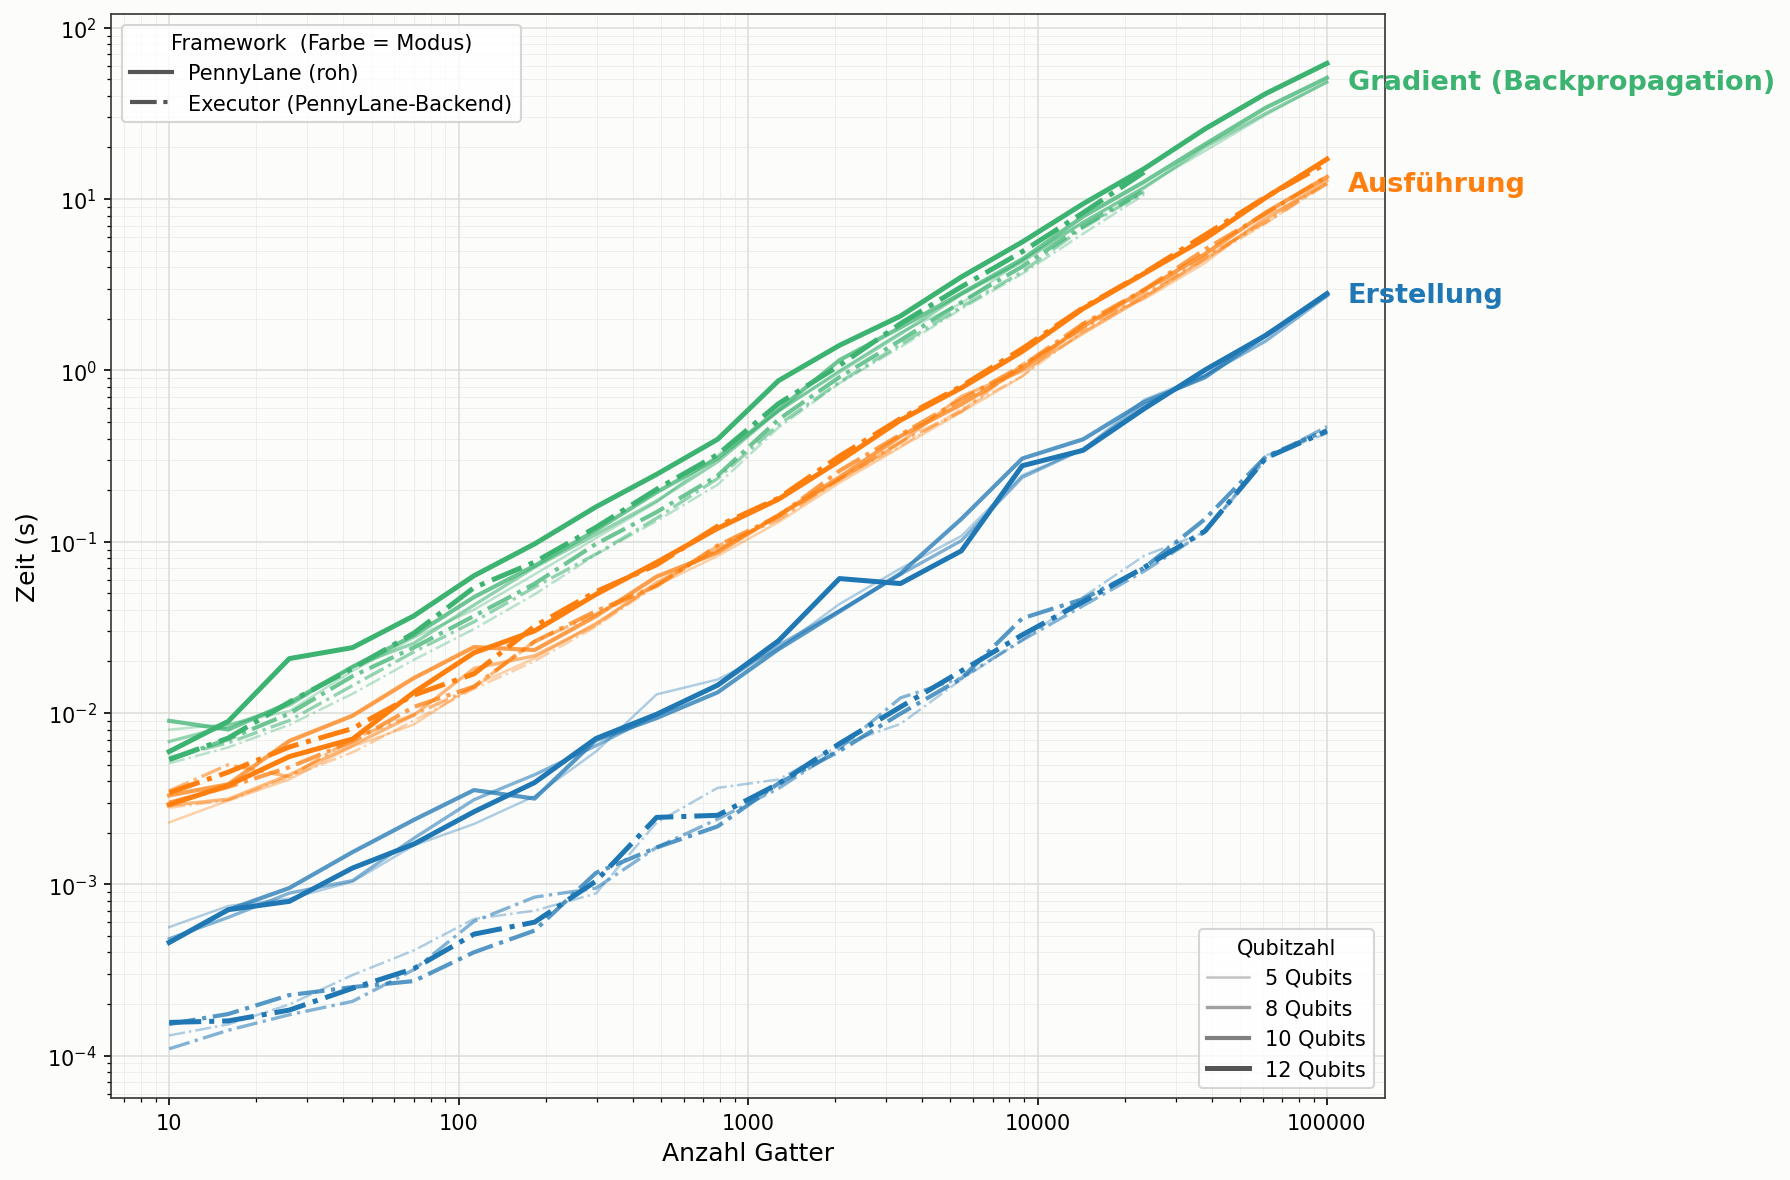
\includegraphics[width=1.1\textwidth]{figures/pennylane_vs_executor_qubits_time_new.png}
    \caption{Laufzeit von nativem \textit{PennyLane} (durchgezogen) und Executor
             mit \textit{PennyLane}-Backend (strichpunktiert)
}
    \label{fig:pennylane-zeit}
\end{figure}

Gemessen wurde über die Qubit-Zahlen 5, 8, 10 und 12 sowie über 20
logarithmisch verteilte Gatterzahlen zwischen 10 und 100\,000, jede Zelle mit
vier Wiederholungen. Abbildung~\ref{fig:pennylane-zeit} zeigt das Ergebnis
doppelt-logarithmisch für alle drei Modi.

Die Qubit-Zahl macht in diesem Bereich nur einen minimalen Unterschied. Die vier
Linien einer Kombination aus Modus und Framework fallen so eng zusammen, dass
sie als ein einziges Band erscheinen. Bei 100\,000 Gattern steigt die native
Laufzeit im Modus \texttt{creation} von $2{,}76$\,s bei 5 Qubits auf
$2{,}80$\,s bei 12 Qubits, im Modus \texttt{execution} von $12{,}1$\,s auf
$17{,}1$\,s. Das ist ein Faktor von $1{,}03$ beziehungsweise $1{,}41$, während
sich der Hilbertraum zwischen beiden Konfigurationen um den Faktor 128
vergrößert. Die Laufzeit wird folglich nicht von der Zustandsvektor-Arithmetik
dominiert, sondern von der pro Gatter anfallenden Python-Arbeit. Nur unter
dieser Voraussetzung wird der Overhead einer zusätzlichen Abstraktionsschicht
überhaupt sichtbar; für deutlich größere Register ist zu erwarten, dass er
relativ zur Simulation verschwindet.

Die Reihen laufen im Modus \texttt{creation} und \texttt{execution} auf beiden
Seiten bis 100\,000 Gatter durch. Im Modus \texttt{gradient} reicht die
Executor-Seite aus Laufzeitgründen nur bis 23\,357 Gatter, die native Seite bis
100\,000. Alle Gradienten-Aussagen beziehen sich daher auf den gemeinsamen
Bereich bis 23\,357 Gatter.

Als Kennzahl dient im Folgenden das geometrische Mittel von
$t_{\mathrm{Executor}}/t_{\mathrm{nativ}}$ über alle Messpunkte ab 1000 Gattern
und alle vier Qubit-Zahlen. Unterhalb von 1000 Gattern liegen die Laufzeiten im
Bereich weniger Millisekunden, wo Einmaleffekte die Verhältnisse verrauschen.

\paragraph*{Erstellung mit erwartbarem Ergebnis}\mbox{}\\
Im Modus \texttt{creation} liegt der Faktor bei $0{,}14$, der Executor ist dort
also rund siebenmal schneller als die native API. Bei 5 Qubits und 100\,000
Gattern stehen $0{,}43$\,s gegen $2{,}76$\,s. Über die vier Qubit-Zahlen ist der
Wert praktisch konstant ($0{,}141$ bis $0{,}146$), und die Steigungen im
Log-Log-Bild sind mit $1{,}07$ bis $1{,}10$ auf beiden Seiten gleich. Es handelt
sich also um einen reinen Vorfaktor und nicht um einen zusätzlichen
Skalierungsterm.

Der Grund liegt darin, dass über die Abstraktionsschicht gar kein vollständiges
Tape entsteht. \verb|ex.transpile_circuit(...)| übersetzt die abstrakte
Gatterliste lediglich in drei parallele Python-Listen mit der
\textit{PennyLane}-Operationsklasse, der Wire-Liste und dem Winkel je Gatter.
Die native Referenz \texttt{qml.\allowbreak workflow.\allowbreak construct\_\allowbreak tape\allowbreak(circuit)()} durchläuft demgegenüber die gesamte Quantenfunktion, instanziiert für jedes Gatter ein
Operationsobjekt, reiht dieses über den Konstruktor in die gerade aktive Queue
ein und setzt daraus ein ausführungsfertiges \texttt{QuantumTape} zusammen.
Tracing, Queuing und Objekterzeugung entfallen beim Executor vollständig.

Diese Zahl ist damit die am wenigsten belastbare der drei und sollte nicht als
Effizienzgewinn gelesen werden, denn beide Seiten leisten hier nicht dieselbe
Arbeit. Das Instanziieren der Operationen holt der Executor bei jeder Ausführung
nach. Der Vorsprung ist keine eingesparte, sondern eine verschobene Arbeit.
Genau deshalb schlägt er im Modus \texttt{execution} nicht mehr durch.

\paragraph*{Ausführung ohne messbaren Overhead}\mbox{}\\
Im Modus \texttt{execution} liegen beide Seiten dicht aufeinander; die
strichpunktierten Executor-Linien liegen innerhalb der Streuung auf den
durchgezogenen nativen Linien. Das geometrische Mittel beträgt $1{,}011$, der
Executor kostet also rund $1$\,\% mehr Laufzeit. Je Qubit-Zahl streut der Wert
zwischen $0{,}99$ und $1{,}03$, in Einzelpunkten zwischen $0{,}82$ und $1{,}12$,
und das Vorzeichen wechselt. Bei 8 und 12 Qubits ist der Executor am rechten
Rand sogar geringfügig schneller ($12{,}31$\,s gegen $12{,}80$\,s
beziehungsweise $16{,}21$\,s gegen $17{,}10$\,s). Ein Overhead von einem Prozent
liegt deutlich unterhalb dessen, was diese Messanordnung auflösen kann; die
belastbare Aussage lautet daher, dass gegenüber \textit{PennyLane} kein
messbarer Overhead entsteht, und nicht, dass er exakt $1{,}1$\,\% beträgt.

Erklärbar ist das über denselben Mechanismus wie bei der Erstellung. Der
Executor spielt bei jedem Aufruf eine vorbereitete Instruktionsliste in einer
Python-Schleife ab, während der native Benchmark die Quantenfunktion erneut
durchläuft und jedes Gatter über die Konstruktoren der Operationsklassen in das
Tape einreiht. Die zusätzliche Ebene des Executors ersetzt hier einen mindestens
ebenso teuren nativen Pfad, statt ihn zu ergänzen.

\paragraph*{Gradientenberechnung mit unerwartetem Ergebnis}\mbox{}\\
Im Modus \texttt{gradient} fällt das Ergebnis unerwartet aus. Das geometrische
Mittel liegt bei $0{,}86$, der Executor ist dort also um 12 bis 15\,\%
\emph{schneller} als die native API, und zwar durchgängig über alle vier
Qubit-Zahlen ($0{,}853$ bis $0{,}878$). Bei 5 Qubits und 23\,357 Gattern stehen
$10{,}60$\,s beim Executor gegen $11{,}83$\,s auf der nativen Seite. Das kann so
nicht stimmen. Der Executor leistet dieselbe Arbeit wie der native Benchmark,
denn Gerät und Schaltkreis sind identisch, und über \verb|diff_method="best"|
rechnet auch er auf \texttt{default.qubit} mit Backpropagation. Zusätzlich
übersetzt er aus der abstrakten Darstellung. Die Abstraktionsschicht müsste
einen Overhead mit sich bringen, kann den nativen Pfad aber nicht unterbieten.

Unabhängig von der Höhe des Faktors ist das Skalierungsverhalten unauffällig.
Beide Seiten wachsen linear in der Gatterzahl, die Steigungen liegen nativ bei
$0{,}99$ bis $1{,}02$ und beim Executor bei $1{,}05$ bis $1{,}07$. Das
bestätigt die Eigenschaft von Backpropagation, dass ein einzelner
Rückwärtsdurchlauf alle Ableitungen liefert und seine Kosten nur von der
Schaltkreisgröße abhängen, nicht von der Parameterzahl; gegenüber der reinen
Ausführung kostet der Gradient lediglich einen konstanten Faktor von etwa 4.
Bemerkenswert ist die kleine, aber über alle vier Qubit-Zahlen gleichgerichtete
Differenz von rund $0{,}05$ im Exponenten. Der Vorsprung des Executors schrumpft
zum rechten Rand hin, von $0{,}86$ im Mittel auf $0{,}89$ bis $0{,}96$ am
letzten gemeinsamen Messpunkt. Der Effekt ist also nicht konstant, sondern
zehrt sich mit wachsender Schaltkreisgröße auf.

\paragraph*{Diskussion des Gradienten-Ergebnisses}\mbox{}\\
Als Ursache für den Wert $0{,}86$ kommt in erster Linie die Laufzeitumgebung in
Betracht, denn die Executor-Gradientenreihe stammt nicht aus demselben Lauf wie
die übrigen Messungen. Der Docker-Container, in dem die Benchmarks ausgeführt
werden, wurde während des ursprünglichen Laufs abgebrochen; die Gradientenreihe
des Executors wurde deshalb am 31.\,07.\,2026 als eigener Lauf nachgezogen,
während alle übrigen Reihen beider Seiten vom 27.\,07.\,2026 stammen. Zwischen
beiden Zeitpunkten wurde das Container-Image neu gebaut, und dabei änderte sich
die \textit{PennyLane}-Version. In der Abhängigkeitsliste war \textit{PennyLane}
zunächst ohne Versionsangabe geführt, sodass die nativen Reihen gegen die zum
Build-Zeitpunkt jeweils neueste Version liefen; für den nachgezogenen
Gradientenlauf des Executors war die Abhängigkeit dagegen auf
\textit{PennyLane}~0.42.3 festgeschrieben. Die beiden Seiten des
Gradienten-Vergleichs wurden also nicht gegen dieselbe Bibliotheksversion
gemessen. Da ein wesentlicher Teil der gemessenen Zeit in \textit{PennyLane}s
eigener Python-Schicht anfällt, also in Tracing, Queuing und Preprocessing des
Tapes, schlagen sich Änderungen an dieser Schicht unmittelbar in der Laufzeit
nieder, und zwar nur auf einer der beiden Seiten des Vergleichs. Wie groß dieser
Beitrag ist, lässt sich nachträglich nicht quantifizieren, da für den früheren
Lauf nur die Abhängigkeit ohne Versionsangabe dokumentiert ist und nicht die
tatsächlich installierte Version.

\newpage
\section{Ergebnisse des Vergleichs von Qiskit und Executor}
\label{sec:ergebnisse-qiskit}

\begin{figure}[H]
    \centering
    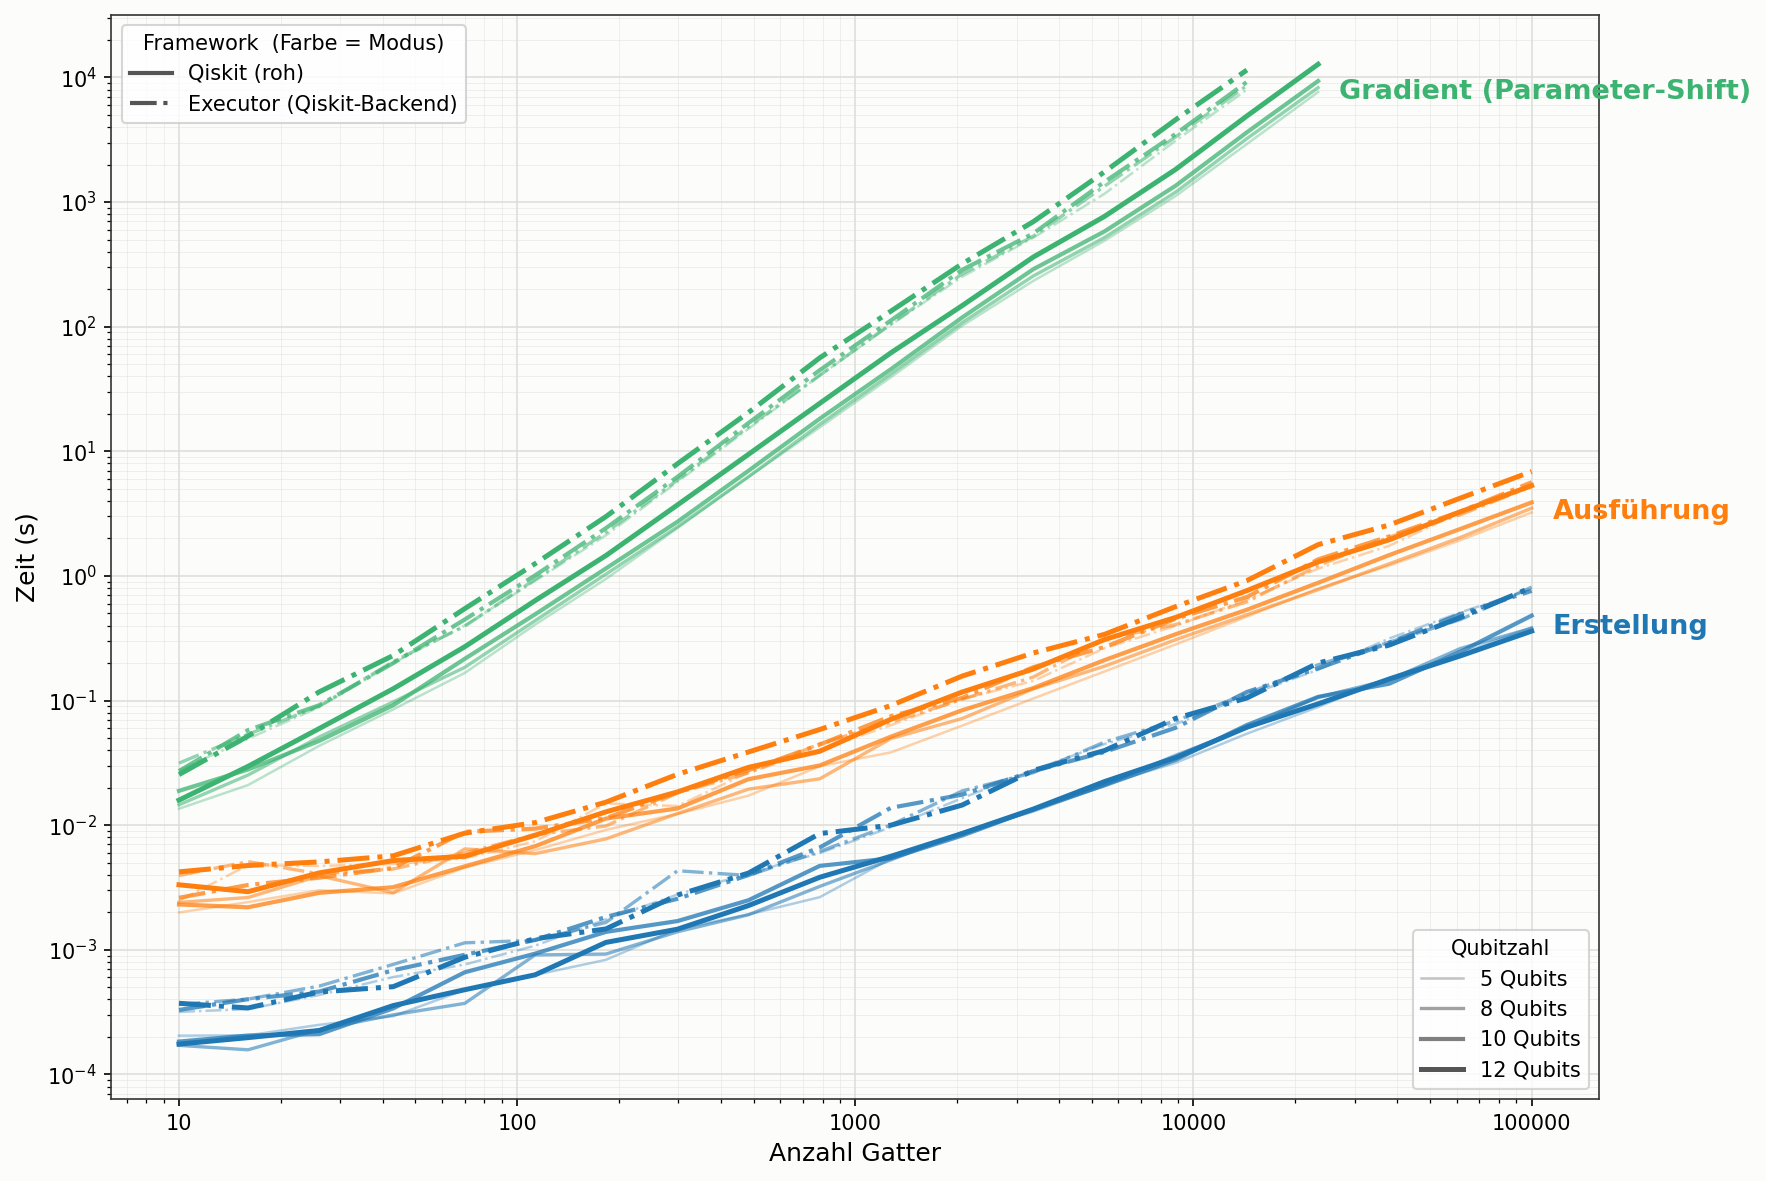
\includegraphics[width=1.1\textwidth]{figures/qiskit_vs_executor_qubits_time.png}
    \caption{Laufzeit von nativem \textit{Qiskit} (durchgezogen) und Executor
             mit \textit{Qiskit}-Backend (strichpunktiert)}
    \label{fig:qiskit-zeit}
\end{figure}

Für das \textit{Qiskit}-Paar gelten dasselbe Messraster und dieselbe Kennzahl
wie oben. Abbildung~\ref{fig:qiskit-zeit} zeigt das Ergebnis in derselben
Auftragung. Das Bild unterscheidet sich in einem Punkt grundlegend von
Abbildung~\ref{fig:pennylane-zeit}. Die strichpunktierten Executor-Linien liegen
in allen drei Modi sichtbar oberhalb der durchgezogenen nativen Linien.
Gegenüber \textit{Qiskit} kostet die Abstraktion also messbar.

Auch hier macht die Qubit-Zahl nur einen minimalen Unterschied, und zwar aus
demselben Grund wie zuvor. Im Modus \texttt{creation} liegen die nativen Zeiten
bei 100\,000 Gattern ohne erkennbaren Trend zwischen $0{,}36$\,s und
$0{,}48$\,s, im Modus \texttt{execution} steigen sie von $3{,}23$\,s bei
5 Qubits auf $5{,}31$\,s bei 12 Qubits. Das ist ein Faktor von $1{,}64$ bei
einem 128-fach größeren Hilbertraum.

Die Gradientenreihe reicht nativ bis 23\,357 Gatter und auf der Executor-Seite
bis 14\,384; die folgenden Gradienten-Aussagen beziehen sich auf den
gemeinsamen Bereich bis 14\,384 Gatter. Der Grund für den früheren Abbruch ist
das Laufzeitbudget, denn eine einzelne Zelle kostet dort bereits mehr als zwei
Stunden.

\paragraph*{Erstellung mit konstantem Faktor 2}\mbox{}\\
Im Modus \texttt{creation} liegt das Verhältnis bei $1{,}97$, die Einzelwerte je
Qubit-Zahl streuen nur zwischen $1{,}93$ und $2{,}02$. Die Steigungen sind mit
$0{,}96$ bis $1{,}02$ auf beiden Seiten praktisch identisch, der Overhead ist
also ein reiner Vorfaktor und kein zusätzlicher Skalierungsterm. Bei 5 Qubits
und 100\,000 Gattern stehen $0{,}79$\,s beim Executor gegen $0{,}39$\,s nativ.

Anders als bei \textit{PennyLane} ist dieser Wert unmittelbar interpretierbar,
denn beide Seiten liefern am Ende dieselbe Datenstruktur, nämlich einen
vollständig befüllten nativen \texttt{QuantumCircuit}. Es wird nichts in eine
spätere Phase verschoben. Der Executor leistet davor zusätzlich die Arbeit der
abstrakten Ebene aus Prüfung jedes Gatters gegen das gemeinsame Vokabular,
Aufbau einer Parameter-Map, Nachschlag der passenden Circuit-Methode und Hashing
für die Memoisierung. Genau diese Zusatzarbeit ist der Faktor 2.

\paragraph*{Ausführung mit Faktor 1,4 und abnehmender Tendenz}\mbox{}\\
Über alle Qubit-Zahlen gemittelt liegt der Overhead bei $1{,}40$. Hier zeigt die
Qubit-Achse als einzige im gesamten Datensatz einen klaren, monotonen Trend. Der
Faktor sinkt von $1{,}51$ bei 5 Qubits über $1{,}44$ und $1{,}38$ auf $1{,}28$
bei 12 Qubits.

Die Erklärung liegt im Nenner und nicht im Zähler. Die absolute Differenz
zwischen beiden Seiten bleibt bei 100\,000 Gattern mit $2{,}07$\,s, $1{,}73$\,s,
$1{,}76$\,s und $1{,}58$\,s über die vier Qubit-Zahlen praktisch konstant,
während die native Laufzeit im selben Schritt von $3{,}23$\,s auf $5{,}31$\,s
wächst. Der Zusatzaufwand des Executors aus Aufbau und Auswertung der
OpTree-Struktur, Deduplizierung und Parameter-Bookkeeping ist reine
Python-Buchhaltung ohne Bezug zur Registergröße. Der relative Overhead wird also
amortisiert, sobald die Simulation teurer wird, und für große Register ist zu
erwarten, dass er weiter gegen 1 läuft.

\paragraph*{Gradientenberechnung mit erwartetem Vorzeichen, aber ohne konstanten
Faktor}\mbox{}\\
Der Gradienten-Modus ist der teuerste Punkt der Paarung mit einem Mittel von
$2{,}40$ und Einzelwerten von $2{,}53$ bei 5 Qubits bis $2{,}22$ bei 12 Qubits.
Anders als bei \textit{PennyLane} fällt das Ergebnis hier in die erwartete
Richtung aus. Der Executor ist langsamer als die native API, so wie es eine
zusätzliche Abstraktionsschicht sein muss. In absoluten Zahlen dauert ein
Gradient bei 5 Qubits und 14\,384 Gattern nativ $2922$\,s und über den Executor
$7985$\,s, was einer Differenz von rund 84 Minuten pro Aufruf entspricht.

Entscheidend ist, dass dieser Faktor als einziger im gesamten Datensatz mit der
Gatterzahl wächst. Über die untere Hälfte des Messbereichs liegt er bei $1{,}91$
bis $2{,}25$, über die obere bei $2{,}23$ bis $2{,}53$ und am letzten
gemeinsamen Messpunkt bei $2{,}34$ bis $2{,}73$. Sichtbar wird das an den
Steigungen im gemeinsamen Bereich, die nativ bei $1{,}74$ bis $1{,}77$ und beim
Executor bei $1{,}78$ bis $1{,}82$ liegen. Die Differenz von rund $0{,}03$ bis
$0{,}04$ im Exponenten ist klein, aber über alle vier Qubit-Zahlen
gleichgerichtet und damit kein Rauschen. Sie passt zu den zwei tiefen
Circuit-Kopien, die der Executor für die Parameter-Shift-Regel je Parameter
anlegt. Jede einzelne kostet $\mathcal{O}(n_{\mathrm{gates}})$ und fällt für
$\mathcal{O}(n_{\mathrm{gates}})$ Parameter an. Zusammen tragen sie damit einen
eigenen quadratischen Term bei, statt den vorhandenen nur zu skalieren.

Dass die gemessenen Exponenten mit etwa $1{,}75$ unterhalb des theoretischen
Werts von 2 liegen, widerspricht dieser Abschätzung nicht. Die Zahl der
Estimator-Läufe wächst exakt linear mit der Gatterzahl, die Kosten eines
einzelnen Laufs steigen im unteren Teil des Messbereichs aber noch unterlinear,
weil dort Fixkosten des Primitivs mitlaufen. Die Steigung nähert sich am rechten
Rand entsprechend an 2 an.

Auf die Einschränkung aus Abschnitt~\ref{sec:ergebnisse-pennylane} ist diese
Paarung nicht angewiesen, denn beide \textit{Qiskit}-Reihen stammen aus
demselben Lauf vom 27.\,07.\,2026 und damit aus demselben Container-Image mit
denselben Bibliotheksversionen. Der Wechsel der \textit{PennyLane}-Version
betrifft sie nicht, und die drei Faktoren sind unabhängig davon interpretierbar.

\chapter{Fazit}
\label{chap:fazit}
\section{Zusammenfassung}

Ziel dieser Arbeit war es, eine framework-unabhängige Abstraktionsschicht für die
Definition parametrisierter Quantenschaltkreise und Observablen zu entwerfen, im
\textit{Executor} zu implementieren und ihren Laufzeit-Overhead gegenüber der
direkten Nutzung der Frameworks zu bestimmen. Dieses Ziel wurde erreicht.

Kapitel~\ref{chap:umsetzung} beantwortet FF1. Die Abstraktion ruht auf vier
framework-unabhängigen Datentypen, deren zulässiges Vokabular zentral in
\texttt{SUPPORTED\_GATES} festgelegt und durch einen Paritätstest über beide
Backends abgesichert ist. Die bisherige Bindung an \textit{Qiskit} wurde damit
aufgelöst, da weder die Basisklassen noch das \textit{PennyLane}-Backend
\textit{Qiskit} importieren.

Kapitel~\ref{chap:vorteile} beantwortet FF2. Als qualitative Vorteile wurden eine
einheitliche Definitionsschnittstelle, die Modularisierbarkeit von Schaltkreisen,
optionale Framework-Abhängigkeiten sowie die Entkopplung von Framework-Versionen
herausgearbeitet. Zugleich wurde gezeigt, dass sich die Ausdrucksstärke der
Schnittstelle notwendigerweise auf die Schnittmenge der unterstützten Frameworks
beschränkt.

Kapitel~\ref{chap:benchmark} beantwortet FF3 mit einem zweigeteilten Befund.
Gegenüber \textit{PennyLane} entsteht in der Ausführung kein messbarer Overhead, da
der \textit{Executor} eine vorbereitete Instruktionsliste abspielt, während die
native Seite den Schaltkreis bei jedem Aufruf neu aufzeichnet. Gegenüber
\textit{Qiskit} kostet die Abstraktion dagegen messbar, und zwar um den Faktor
$1{,}97$ bei der Erstellung, $1{,}40$ bei der Ausführung und $2{,}40$ bei der
Gradientenberechnung. Der relative Overhead der Ausführung nimmt mit wachsender
Qubit-Zahl ab, da der Zusatzaufwand aus reiner Python-Buchhaltung besteht und nicht
von der Registergröße abhängt. Allein bei der Gradientenberechnung über
\textit{Qiskit} wächst der Faktor mit der Gatterzahl, was auf die tiefen
Schaltkreiskopien der Parameter-Shift-Regel zurückgeht. Der gemessene Vorsprung des
\textit{Executors} bei der Gradientenberechnung über \textit{PennyLane} bleibt wegen
abweichender Bibliotheksversionen zwischen beiden Messläufen nur eingeschränkt
belastbar.

Der gemessene Mehraufwand fällt gegenüber dem gewonnenen Nutzen gering aus.
Gegenüber \textit{PennyLane} arbeitet der \textit{Executor} auf dem Niveau der
nativen API, und gegenüber \textit{Qiskit} bewegt sich der Overhead in der
Ausführung in einem Bereich, der sich mit wachsender Registergröße weiter
angleicht, da der Zusatzaufwand nicht mit der Qubit-Zahl skaliert. Er beschränkt
sich damit auf einen konstanten Anteil an Python-Arbeit, dem eine einmalige, über
sämtliche Backends hinweg wiederverwendbare Problembeschreibung gegenübersteht.
Gerade dort, wo Laufzeit tatsächlich ins Gewicht fällt, also bei großen Registern
und rechenintensiven Simulationen, verliert der Overhead zusätzlich an Bedeutung.
Die in Kapitel~\ref{chap:vorteile} beschriebenen Vorteile, insbesondere die
kontrollierte Vergleichbarkeit von Backends, die optionalen
Framework-Abhängigkeiten und die Stabilität über Versionswechsel hinweg, wiegen
diesen Anteil in der Praxis auf.

Damit sind alle drei Forschungsfragen beantwortet.
% ----------------------------------------------------------------
\newpage
\section{Ausblick}
\label{sec:ausblick}
Der Executor im Allgemeinen und die Abstraktionsschicht können noch
weiterentwickelt werden, um Anbindungen an weitere Backends zu schaffen. Im
Moment werden nur \textit{PennyLane} und \textit{Qiskit} als API-Endpunkte
unterstützt, was bereits eine gute Basis bildet. Darüber hinaus ist die Grundlage
für eine Implementierung von \textit{Qulacs} und der Pauli-Propagation bereits
gegeben. Bei diesen fehlt jedoch noch die Umwandlung der abstrakten Schaltkreis-
und Observablen-Objekte in die Framework-spezifischen Repräsentationen. Auch
weitere Frameworks wie \textit{Cirq}, \textit{Braket SDK} oder \textit{Q\#} wären
sinnvolle Ergänzungen. Damit würde der Executor ein größeres Ökosystem
unterstützen und mehr Nutzerinnen und Nutzer ansprechen, die diese Backends
einsetzen.

Zudem orientiert sich die Abstraktionsschicht derzeit an der NISQ-Ära, also an verrauschten Quantencomputern ohne Fehlerkorrektur~\cite{preskill2018quantum}. Ihr Entwurf ist daher auf parametrisierte Schaltkreise sowie die Berechnung von Erwartungswerten und Gradienten ausgelegt. Perspektivisch wird jedoch das fehlertolerante Quantencomputing wichtiger, das mit fehlerkorrigierten logischen Qubits arbeitet. Diese Technologie steht allerdings noch am Anfang und ist bisher nicht praktisch nutzbar, sodass eine Anpassung der Abstraktionsschicht erst mit der Verfügbarkeit entsprechender Backends sinnvoll wird.

% Was sind sinnvolle nächste Schritte?
% Offen gebliebene Fragen, mögliche Erweiterungen,
% Verbesserungspotenziale, Anknüpfungspunkte für weitere Arbeiten.

%% ---- Back Matter -------------------------------------------
\printbibliography[title={Literaturverzeichnis}]

\appendix
%% ============================================================
%%  07_anhang.tex
%%  Kapitel A: Anhang
%% ============================================================

\chapter{Anhang}
\label{chap:anhang}

% Alles, was den Lesefluss im Hauptteil gestört hätte,
% aber zur Vollständigkeit gehört.

% ----------------------------------------------------------------
\section{Zugang zum Quellcode}
\label{sec:anhang_code}


Der im Rahmen dieser Arbeit entwickelte Quellcode ist öffentlich über GitHub
verfügbar und gliedert sich in zwei Repositories.


Das erste Repository enthält die Implementierung der Abstraktionsschicht
\texttt{qc\_executor}, welche die einheitliche Ansteuerung der verschiedenen
Backends kapselt:


\url{https://github.com/flaqship/qc-executor}


Das zweite Repository umfasst das Benchmarking-System, mit dem die vorgestellten Performance-Messungen
durchgeführt wurden:

\url{https://github.com/dfaigle/benchmarking-system}

% Längere Listings, die im Hauptteil zu viel Platz brauchen.


\newpage
\section{Eidesstattliche Erklärung}
\addcontentsline{toc}{chapter}{Eidesstattliche Erklärung}
\thispagestyle{empty}

Ich erkläre hiermit an Eides statt, dass ich die vorliegende
Bachelor-Thesis mit dem Titel

\begin{center}
  \emph{\ThesisTitel}
\end{center}

selbstständig und ohne Benutzung anderer als der angegebenen Hilfsmittel
angefertigt habe.

Bei der Erstellung dieser Arbeit wurden KI-basierte Werkzeuge unterstützend
eingesetzt, und zwar zur Rechtschreib- und Formulierungshilfe, beim Finden
von Quellen sowie zur Unterstützung beim Programmieren. Die inhaltliche
Verantwortung für die Arbeit liegt vollständig bei mir.

Alle Stellen, die wörtlich oder sinngemäß aus veröffentlichten oder nicht
veröffentlichten Schriften entnommen wurden, sind als solche kenntlich
gemacht. Die Arbeit ist in gleicher oder ähnlicher Form noch nicht als
Prüfungsarbeit eingereicht worden.

Ich bin mir bewusst, dass eine falsche Erklärung rechtliche Folgen haben wird.
\vspace{3cm}

\noindent
\begin{tabular}{p{6cm}p{1cm}p{6cm}}
  Heilbronn, \ThesisDatum & & \\[0.3cm]
  \cline{1-1}\cline{3-3}\\[-0.5cm]
  Ort, Datum              & & \ThesisAutor
\end{tabular}


%% ============================================================
%%  08_eidesstattliche_erklaerung.tex
%%  Pflichtbestandteil jeder Bachelor-Thesis an der HHN
%% ============================================================


\end{document}
